%%%%%%%%%%%%%%%%%%%%%%%%%%%%%%%%%%%%%%%%%
% Structured General Purpose Assignment
% LaTeX Template
%
% Template Name: Anthony
% The template was named after my friend Anthony.
% Strong inspired by Apache Hadoop and Java (programming language)
%
% Author: Ang LEE
%
% Blog: http://angli.me/
%
% Github: https://github.com/leeang/
%
%%%%%%%%%%%%%%%%%%%%%%%%%%%%%%%%%%%%%%%%%

%----------------------------------------------------------------------------------------
%	CONSTANTS
%----------------------------------------------------------------------------------------

\newcommand{\hmwkTitle}{MATLAB Project Report}			% Assignment title
\newcommand{\hmwkClass}{Signal Processing}				% Course name
\newcommand{\hmwkClassTime}{}							% Workshop time
\newcommand{\hmwkClassInstructor}{}						% Tutor name
\newcommand{\hmwkAuthorName}{Ang LEE}					% Student name

\newcommand{\hmwkGraphicsPath}{img/}					% Graphics path
\newcommand{\hmwkCodePath}{code/}						% Code path

%----------------------------------------------------------------------------------------
%	TEMPLATE
%----------------------------------------------------------------------------------------

\documentclass{article}

\usepackage{fancyhdr}	% Required for custom headers
\usepackage{lastpage}	% Required to determine the last page for the footer
\usepackage{extramarks} % Required for headers and footers
\usepackage{graphicx}	% Required to insert images
\graphicspath{\hmwkGraphicsPath}

\usepackage{float}
\usepackage{epstopdf}	% Required to insert .eps images
\usepackage{amssymb}
\usepackage{amsmath}
\usepackage[hidelinks]{hyperref}
\usepackage{tabu}		% Required to insert table of certain width

% MATLAB syntax highlighting
\usepackage{color}		% Required to define colors
\definecolor{commentColor}{RGB}{34,139,34}
\definecolor{stringColor}{RGB}{160,32,240}
\usepackage{listings}
\lstset{
	inputpath=\hmwkCodePath,
	language=Matlab,
	basicstyle=\footnotesize\ttfamily,
	keywordstyle=\color{blue},
	stringstyle=\color{stringColor},
	commentstyle=\usefont{T1}{pcr}{m}{n}\color{commentColor},
	breaklines=true,
	showstringspaces=false,
	numbers=left,
	numberstyle=\scriptsize,
	firstnumber=1,
	numberfirstline=true,
	stepnumber=5,
	frame=leftline
}

% change \textbf textbf
\definecolor{bfcolor}{RGB}{221,75,57}
\DeclareTextFontCommand{\textbf}{\bfseries\color{bfcolor}}

% change \texttt color
\definecolor{ttcolor}{RGB}{0,103,179}
\DeclareTextFontCommand{\texttt}{\ttfamily\color{ttcolor}}

% change headings color
\usepackage{sectsty}
\definecolor{sectioncolor}{RGB}{0,102,33}
\sectionfont{\color{sectioncolor}\sffamily}
\definecolor{subsectioncolor}{RGB}{26,131,171}
\subsectionfont{\color{subsectioncolor}\sffamily}
\definecolor{subsubsectioncolor}{RGB}{0,51,102}
\subsubsectionfont{\color{subsubsectioncolor}\sffamily}

% Margins
\topmargin=-0.45in
\evensidemargin=-0.5in
\oddsidemargin=-0.5in
\textwidth=7.5in
\textheight=9.0in
\headsep=0.25in

\linespread{1.1}		% Line spacing

% Set up the header and footer
\pagestyle{fancy}
\lhead{\hmwkTitle} % Header Left 
\chead{\hmwkAuthorName} % Header Center
\rhead{\hmwkClass} % Header Right
\lfoot{\url{https://github.com/leeang/Signal-Processing}} % Footer Left
\cfoot{} % Footer Center
\rfoot{Page\ \thepage\ of\ \pageref{LastPage}} % Footer Right
\renewcommand\headrulewidth{0.4pt} % Size of the header rule
\renewcommand\footrulewidth{0.4pt} % Size of the footer rule

\setlength\parindent{0pt} % Removes all indentation from paragraphs

%----------------------------------------------------------------------------------------
%	Problem and Section
%----------------------------------------------------------------------------------------

\newenvironment{homeworkProblem}[1]{
	\section{#1}
	}{
}
\newenvironment{homeworkSection}[1]{
	\subsection{#1}
	}{
}
\newcommand{\problemAnswer}[1]{
	\noindent\framebox[\columnwidth][c]{
		\begin{minipage}{0.98\columnwidth}
			#1
		\end{minipage}
	}
}

%----------------------------------------------------------------------------------------
%	Document
%----------------------------------------------------------------------------------------

\begin{document}

\newpage

%----------------------------------------------------------------------------------------
%	Analysis
%----------------------------------------------------------------------------------------

\begin{homeworkProblem}{$r_s[n]$ analysis}

Student number: 7 and 4. Hence we use \texttt{projsignal\textit{m}.mat} where $m=1$, carrier frequency $F_c$ = 12.288 kHz.

%--------------------------------------------

\begin{figure}[H]
\centering
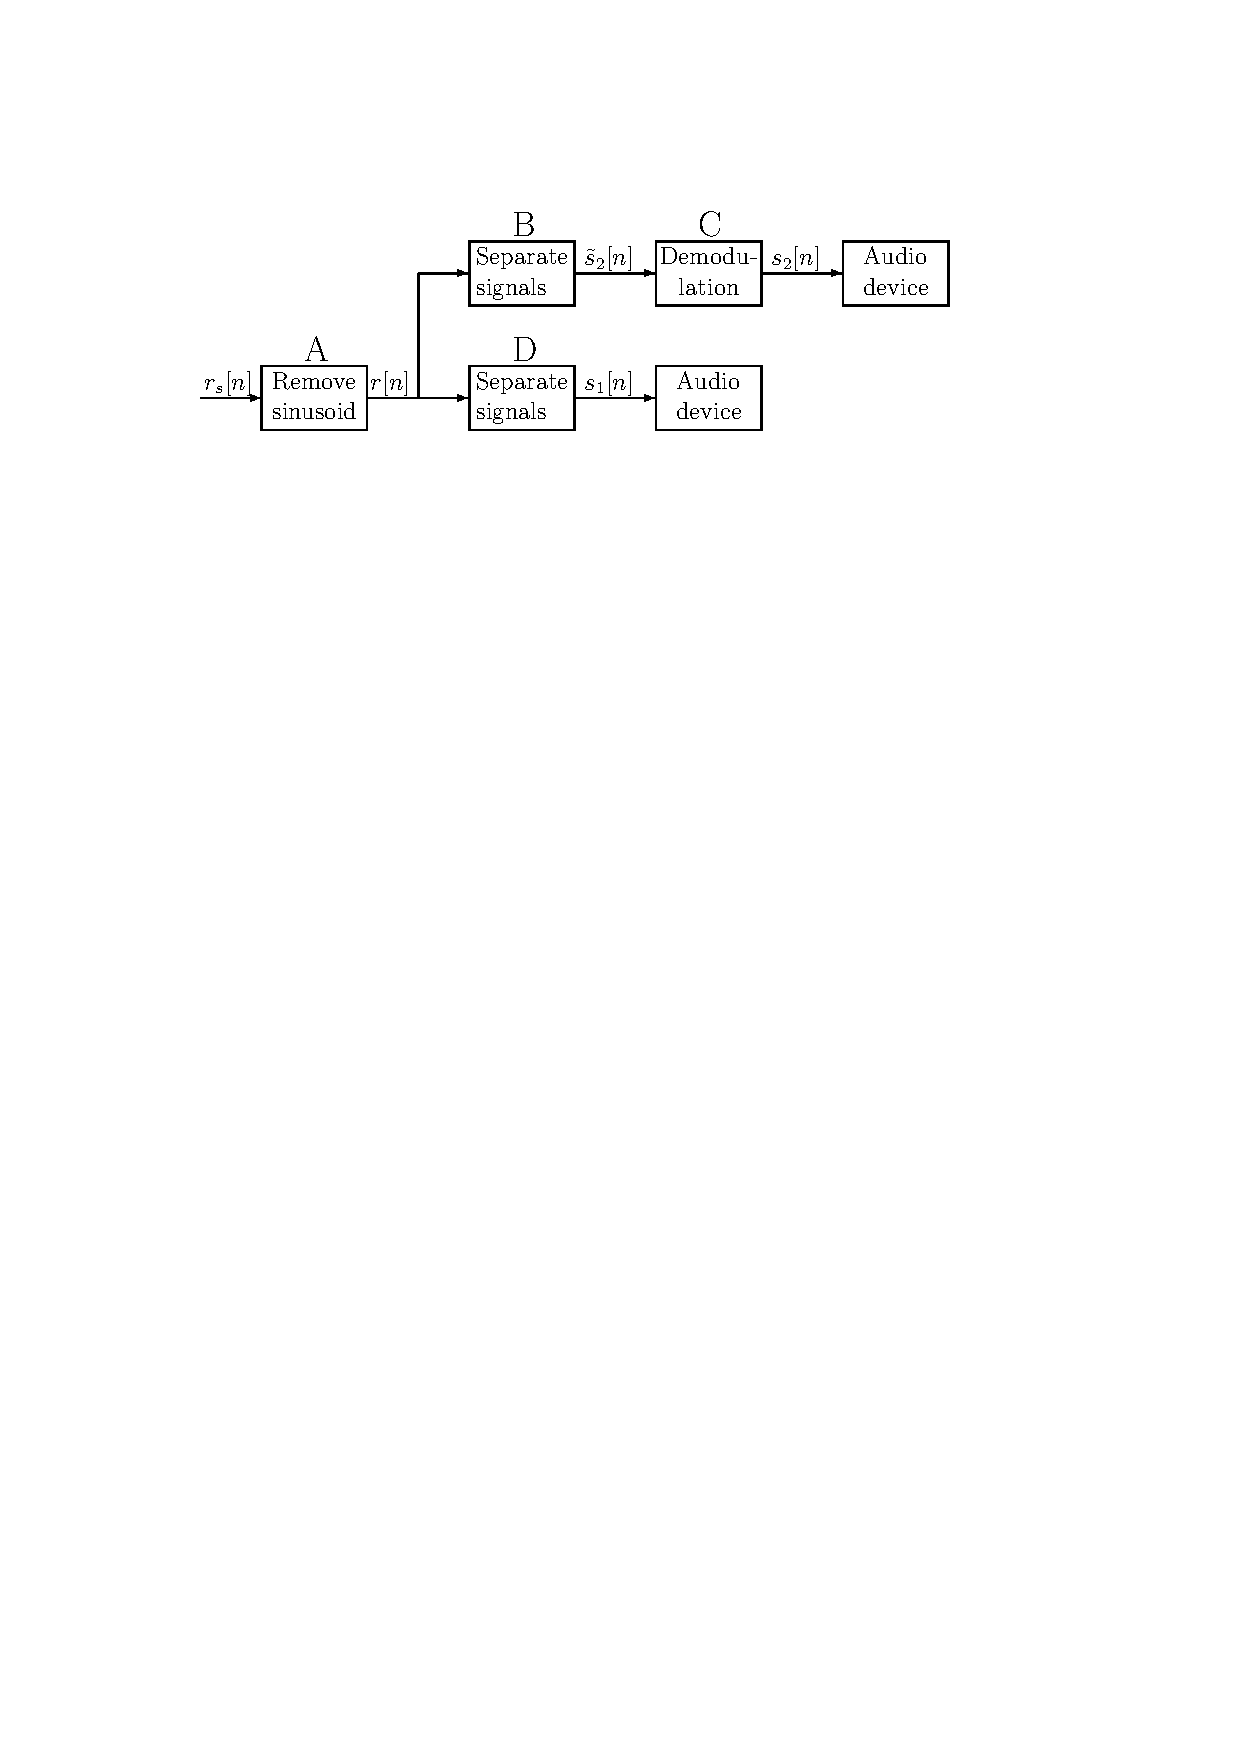
\includegraphics[width=3.9in]{signal-removal-and-separation}
\caption{Signal removal and separation}
\label{signal-removal-and-separation}
\end{figure}

In Figure \ref{signal-removal-and-separation}, the signal $r_s[n]$ is made up of three components
\begin{equation}
r_s[n] = r_1[n] + r_2[n] + w[n]
\end{equation}
$r_1[n]$ and $r_2[n]$ are the two important signal components and they occupy two separate frequency bands. $r_1[n]$ has a bandwidth of 4096 Hz, and $r_2[n]$ is a DSB-SC (double side band, suppressed carrier) modulated signal. The carrier frequency is $F_c$ kHz, and the bandwidth of the original signal is 4096 Hz. $w[n]$ is a sinusoidal disturbance signal. The sampling frequency of $r_s[n]$ is 32.768 kHz.\\

In block A the sinusoid $w[n]$ is removed. The two signal components of $r[n]$ are then separated in block B and D such that output of block B, $\tilde{s}_2[n]$ contains the high frequency signal, and the output of block D contains the low frequency signal. The high frequency signal $\tilde{s}_2[n]$ is demodulated in block C, so that the original signal is recovered.

%--------------------------------------------

\begin{figure}[H]
\begin{minipage}[t]{0.5\linewidth}
\centering
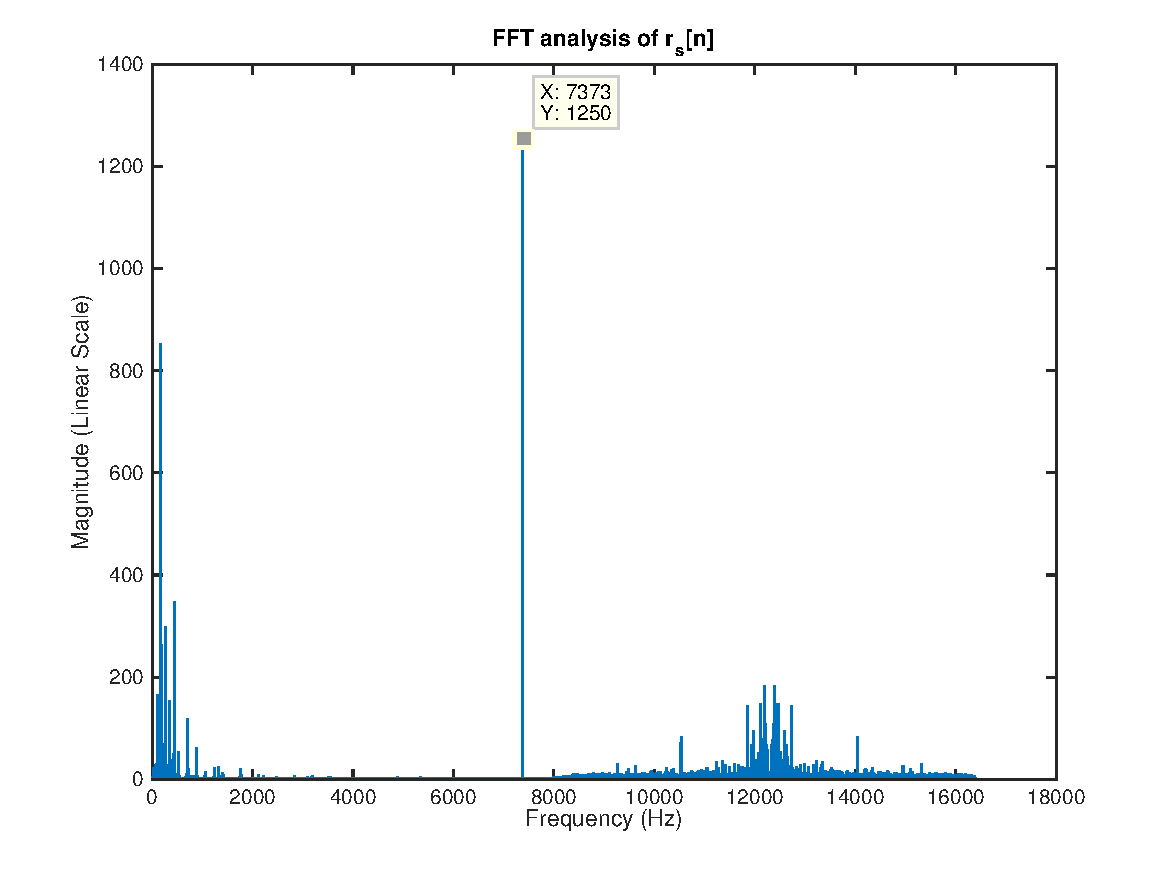
\includegraphics[width=3.3in]{rs_FFT_linear}
\caption{$r_s[n]$ in frequency domain (Linear scale)}
\label{rs_FFT_linear}
\end{minipage}
\begin{minipage}[t]{0.5\linewidth}
\centering
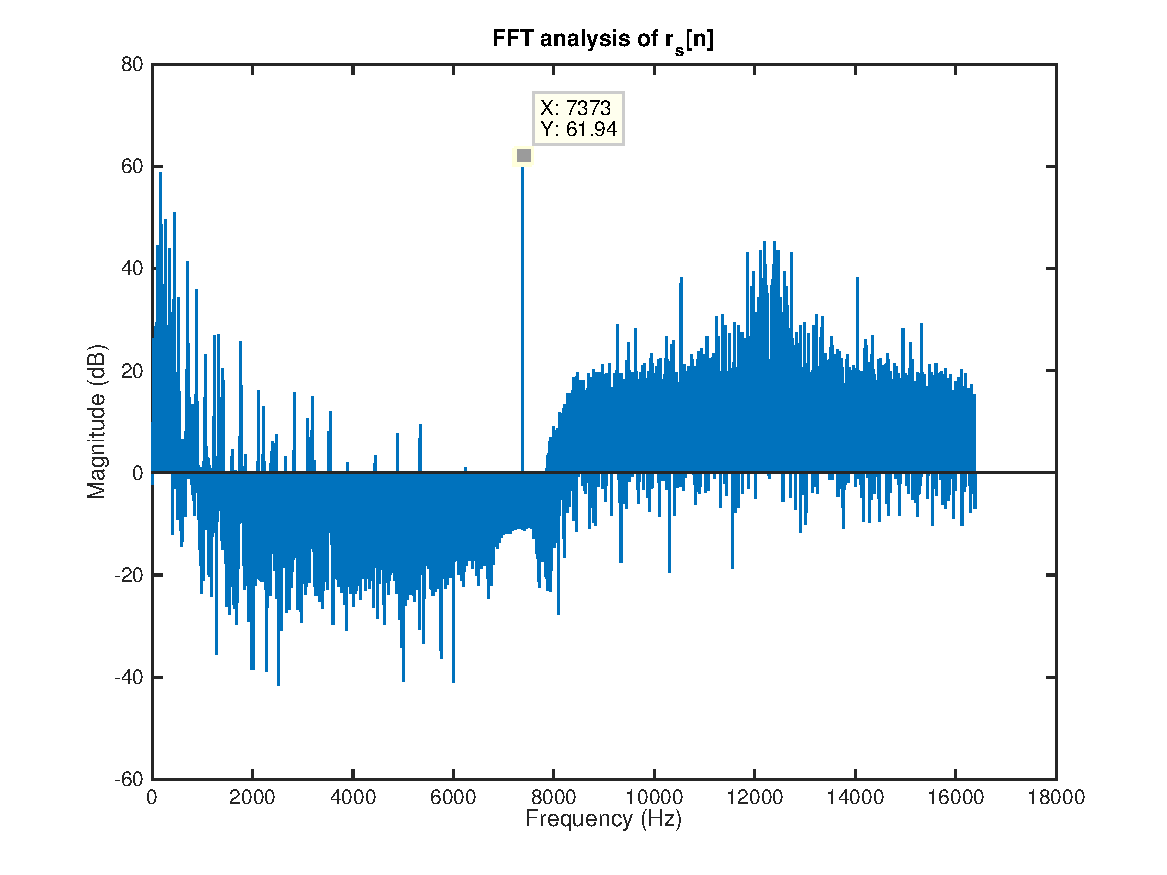
\includegraphics[width=3.3in]{rs_FFT_dB}
\caption{$r_s[n]$ in frequency domain (dB)}
\label{rs_FFT_dB}
\end{minipage}
\end{figure}

It can be clearly seen in Figure \ref{rs_FFT_linear}, the frequency of $w[n]$ is 7372.8 Hz ($0.45\pi$ rad/sample).\\

Assuming $r_2(t)$ is the DSB-SC modulated signal of $m(t)$
\begin{equation}\label{r2_fourier}
r_2(t) = m(t) \cos(2 \pi F_c t) \leftrightarrow R_2(f) = \frac{1}{2} [M(f + F_c) + M(f - F_c)]
\end{equation}
Hence, $r_2[n]$ has a bandwidth of $[F_c-4096\text{ Hz}, F_c+4096\text{ Hz}]$.
\begin{equation}\label{DSBSC-BW}
B_w = [8192 \text{ Hz}, 16384 \text{ Hz}]
\end{equation}

Note that: the carrier signal with the phase $\phi$, $v_c(t) = \cos(2 \pi F_c t + \phi)$ will have the same magnitude - frequency spectra. (The phase - frequency spectra are different.)\\

Define
\begin{equation}
y(t) := r_2(t) \cos(2 \pi F_c t)
\end{equation}
Similar to Eq. \ref{r2_fourier}
\begin{equation}
y(t) \leftrightarrow Y(f) = \frac{1}{2} [R_2(f + F_c) + R_2(f - F_c)]
\end{equation}
\begin{equation}
Y(f) = \frac{1}{2} M(f) + \frac{1}{4} M(f + 2F_c) + \frac{1}{4} M(f - 2F_c)
\end{equation}
Apparently, multiplying the DSB-SC signal with the carrier signal yields a scaled version of the original message signal plus a higher frequency term.\\

To sum up, block A is a notch filter ($w[n]$ frequency: 7372.8 Hz, i.e. $0.45\pi$ rad/sample); block D is a lowpass filter ($r_1[n]$ frequency band: [0, 4096 Hz]); block B is a highpass filter ($r_2[n]$ frequency band: [8192 Hz, 16384 Hz]); block C contains a lowpass filter (bandwidth of interest: [0, 4096 Hz]).\\

The demodulation oscillator's phase $\phi_2$ must be exactly the same as modulation oscillator's $\phi_1$, otherwise, attenuation will occur. To see this effect, take demodulation signal with small phase deviations $\theta$ from the modulation signal: $\cos(2 \pi F_c t + \theta)$.\\

The resultant signal is attenuated by a constant factor $\cos(\theta)$.
\begin{align*}
& m(t) \cos(2 \pi F_c t) \cos(2 \pi F_c t + \theta)\\
&= \frac{1}{2} m(t) \cos(\theta) + \frac{1}{2} m(t) \cos(2 \cdot 2\pi F_c t + \theta)\\
& \xrightarrow{\text{After low pass filter}} \frac{1}{2} m(t) \cos(\theta)
\end{align*}
Our goal is to make $\cos(\theta) \to 1$, in other words, $\theta \to 0$.\\

Define the demodulation carrier signal:
\begin{equation}\label{demodulation_carrier}
v_c(t) = \cos(2 \pi F_c t + \phi_2)
\end{equation}

In order to obtain the $\phi_2$ that minimizes $|\theta| = |\phi_1 - \phi_2|$, different $\phi_2$ will be tested until the largest amplitude of demodulated signal is found. Function \texttt{find\_phi(s2\_tilde)} is programmed to find optimal $\phi_2$ (available on page \pageref{find_phi}).

%--------------------------------------------

\end{homeworkProblem}

%----------------------------------------------------------------------------------------
%	FIR filters design
%----------------------------------------------------------------------------------------

\begin{homeworkProblem}{FIR filters design}

%--------------------------------------------

\begin{homeworkSection}{Block A Notch filter}

\subsubsection{Specification}
Method: \textbf{Parks-McClellan} optimal FIR filter design\\
Passband: [0, 6872.8 Hz] and [7872.8 Hz, $+\infty$)\\
Stopband: [7371.8 Hz, 7373.8 Hz]\\
Passband ripple: 0.005 (smaller than 0.01 for further cascade)\\
Stopband ripple: 0.001 (-60 dB)\\

The lowest order can be calculated by \texttt{firpmord()} function.
\begin{equation}
N = 184
\end{equation}

\begin{figure}[H]
\begin{minipage}[t]{0.5\linewidth}
\centering
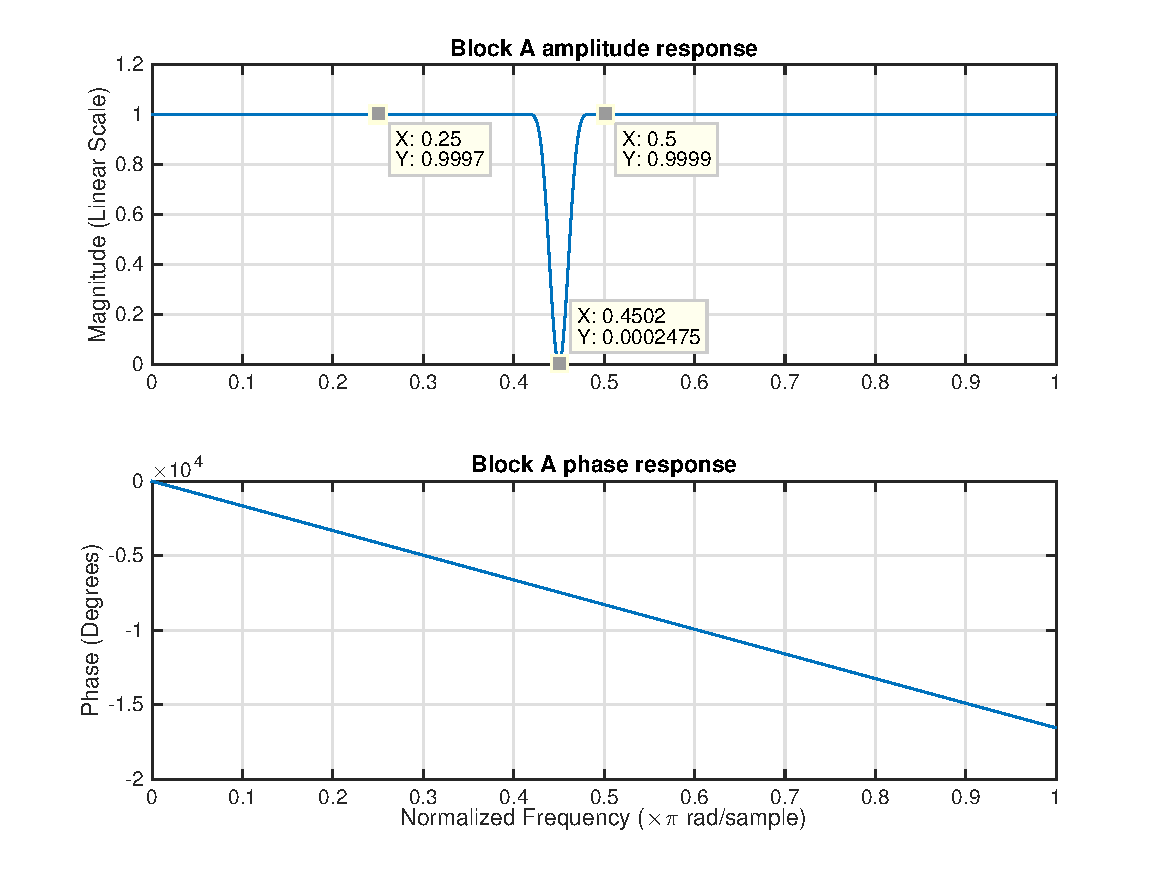
\includegraphics[width=3.3in]{BlockA-Response-FIR}
\caption{Block A response}
\label{BlockA-Response-FIR}
\end{minipage}
\begin{minipage}[t]{0.5\linewidth}
\centering
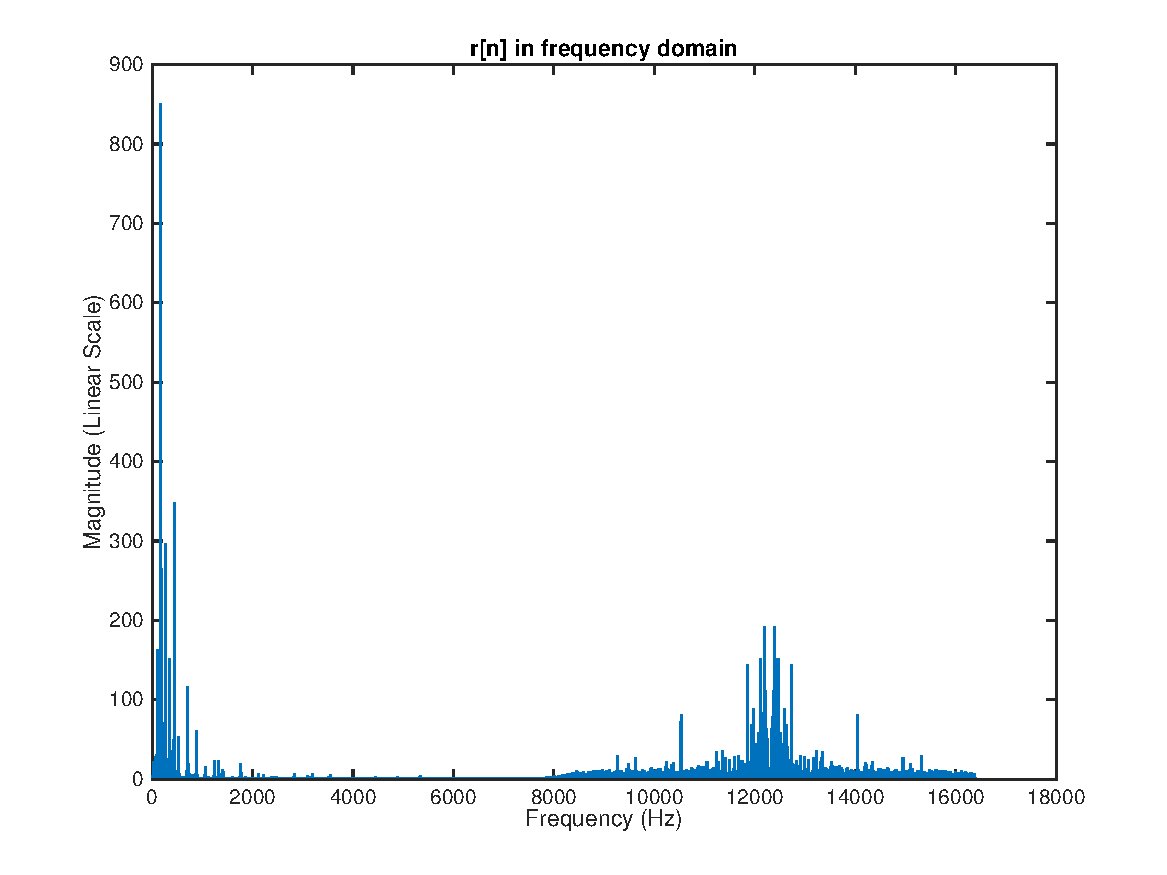
\includegraphics[width=3.3in]{r_FFT-FIR}
\caption{$r[n]$ in frequency domain}
\label{r_FFT-FIR}
\end{minipage}
\end{figure}

As can be seen in Figure \ref{BlockA-Response-FIR} and Figure \ref{r_FFT-FIR}, $w[n]$ at 7372.8 Hz ($0.45\pi$ rad/sample) has been attenuated by $20 \log_{10}(0.0002475)$ = -72.1285 dB $<$ -60 dB. Also, the notch filter has linear phase.

\end{homeworkSection}

%--------------------------------------------

\begin{homeworkSection}{Block D Lowpass filter}

\subsubsection{Specification}
Method: \textbf{Parks-McClellan} optimal FIR filter design\\
Passband: [0, 4096 Hz]\\
Stopband: [4596 Hz, $+\infty$)\\
Passband ripple: 0.005 (smaller than 0.01 because of cascade)\\
Stopband ripple: 0.01 (-40 dB)\\

The lowest order can be calculated by \texttt{firpmord()} function.
\begin{equation}
N = 141
\end{equation}

%--------------------------------------------

\subsubsection{Frequency Response \& Output}
\begin{figure}[H]
\begin{minipage}[t]{0.33\linewidth}
\centering
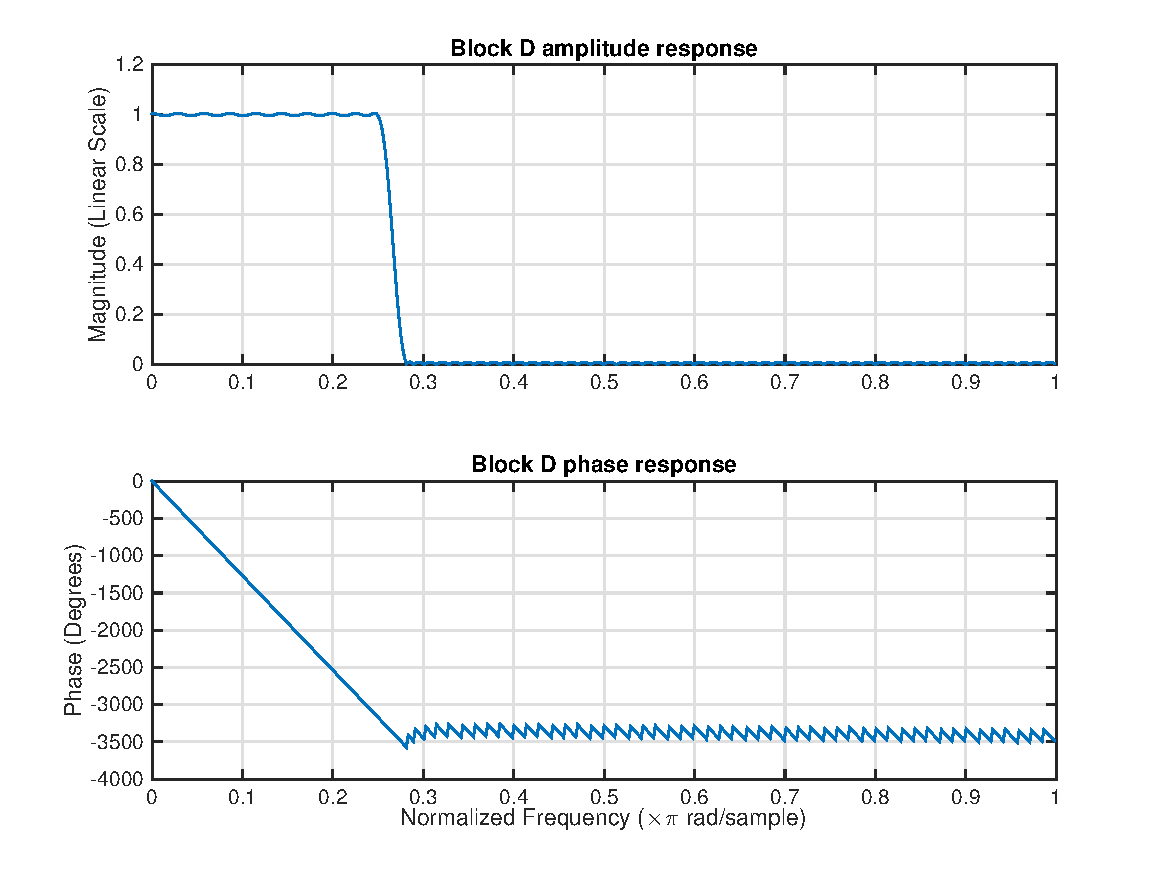
\includegraphics[width=2.5in]{BlockD-Response-FIR}
\caption{Block D response}
\label{BlockD-Response-FIR}
\end{minipage}
\begin{minipage}[t]{0.33\linewidth}
\centering
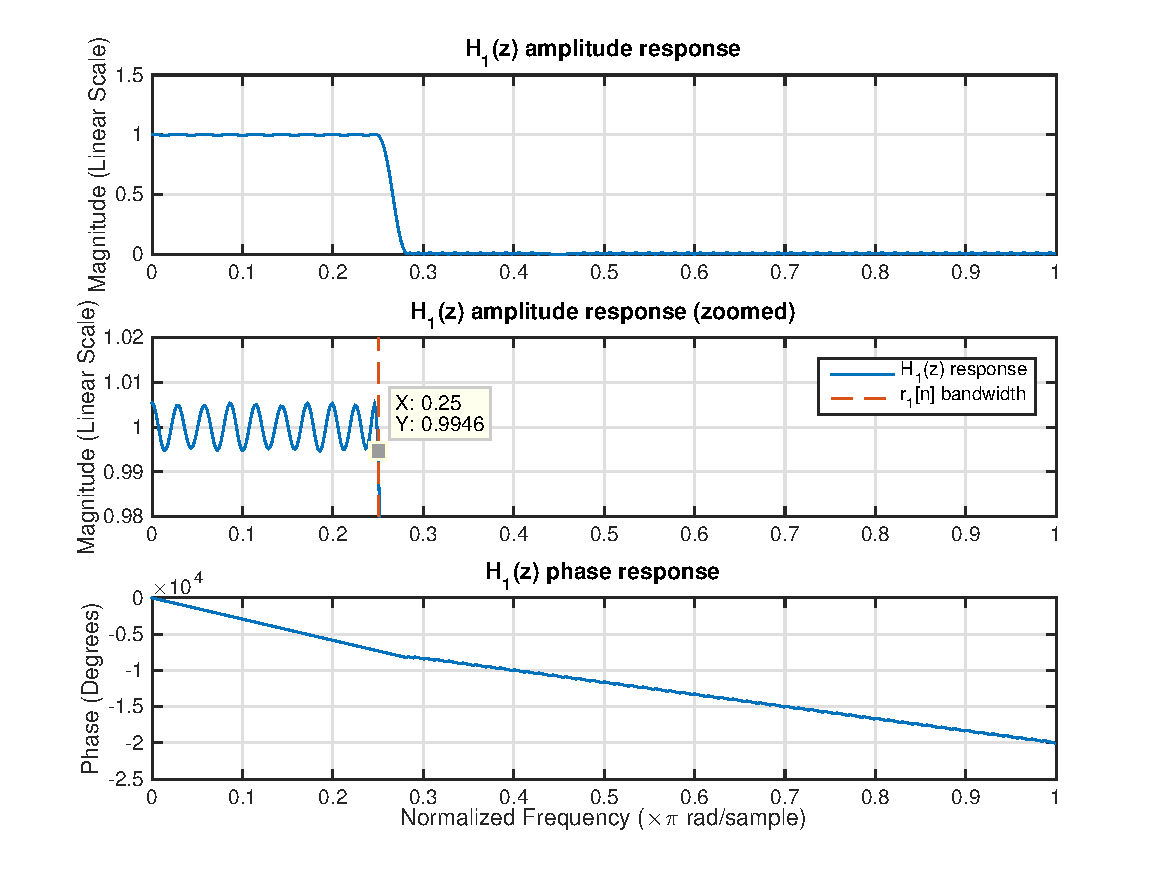
\includegraphics[width=2.5in]{H1-Response-FIR}
\caption{$H_1(z)$ Response}
\label{H1-Response-FIR}
\end{minipage}
\begin{minipage}[t]{0.33\linewidth}
\centering
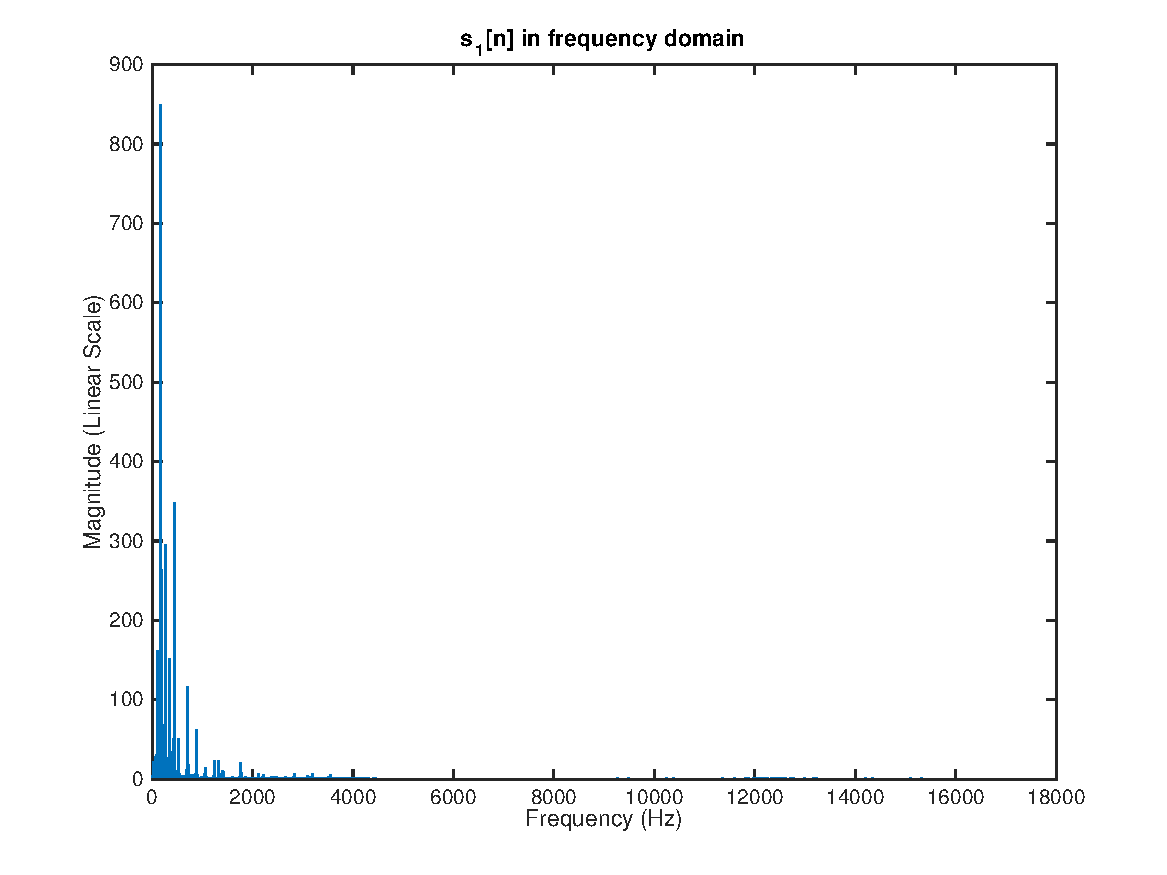
\includegraphics[width=2.5in]{s1-FIR}
\caption{$s_1[n]$ in frequency domain}
\label{s1-FIR}
\end{minipage}
\end{figure}

In Fig. \ref{BlockD-Response-FIR}, Block D has linear phase. In Fig. \ref{H1-Response-FIR}, $H_1(z)$ has ripple less than 0.01. In Fig. \ref{s1-FIR}, high frequency components have been successfully filtered.\\

\textbf{$H_1(z)$ is the filter obtained by cascading the filters in block A and D}.

\end{homeworkSection}

%--------------------------------------------

\begin{homeworkSection}{Block B Highpass filter}

\subsubsection{Specification}
Method: \textbf{Parks-McClellan} optimal FIR filter design\\
Stopband: [0, 7692 Hz]\\
Passband: [8192 Hz, $+\infty$)\\
Stopband ripple: 0.01 (-40 dB)\\
Passband ripple: 0.005 (smaller than 0.01 because of cascade)\\

The lowest order can be calculated by \texttt{firpmord()} function.
\begin{equation}
N = 140
\end{equation}

%--------------------------------------------

\subsubsection{Frequency Response \& Output}
\begin{figure}[H]
\begin{minipage}[t]{0.33\linewidth}
\centering
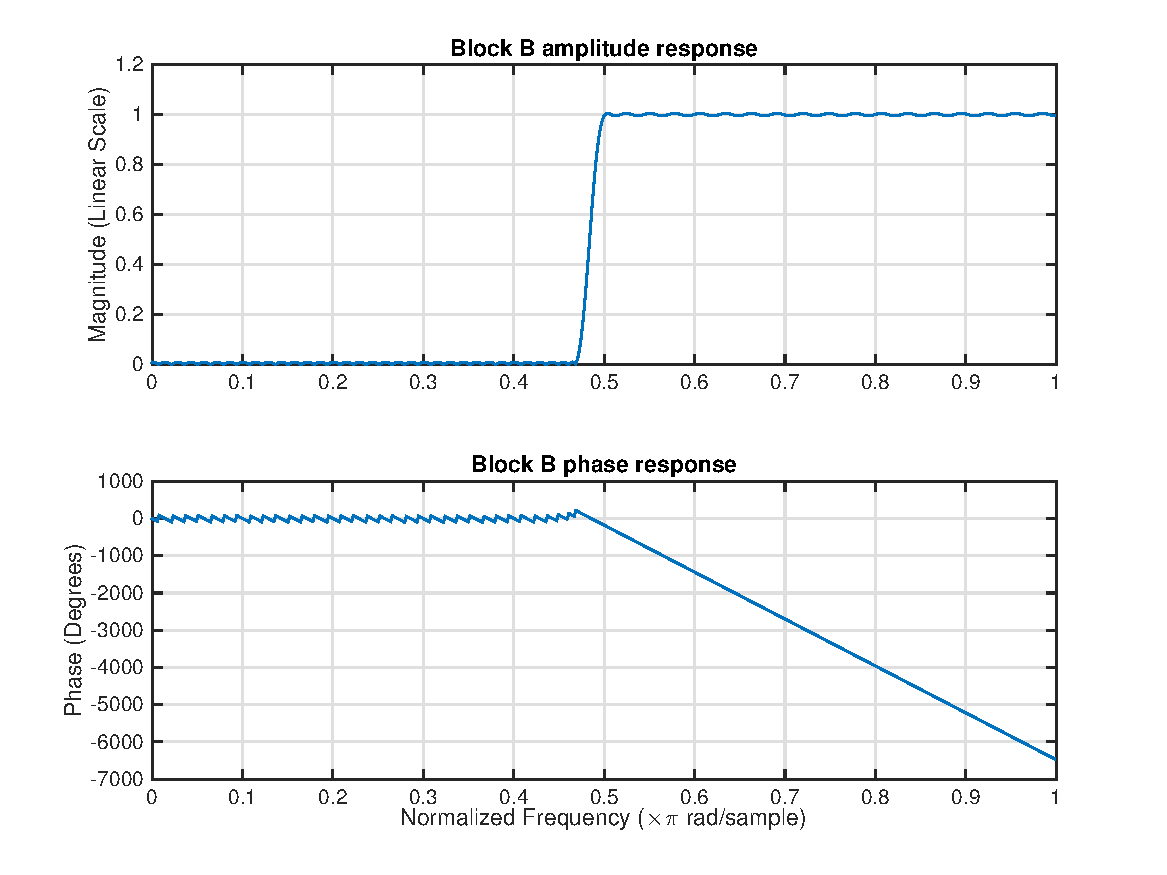
\includegraphics[width=2.5in]{BlockB-Response-FIR}
\caption{Block B response}
\label{BlockB-Response-FIR}
\end{minipage}
\begin{minipage}[t]{0.33\linewidth}
\centering
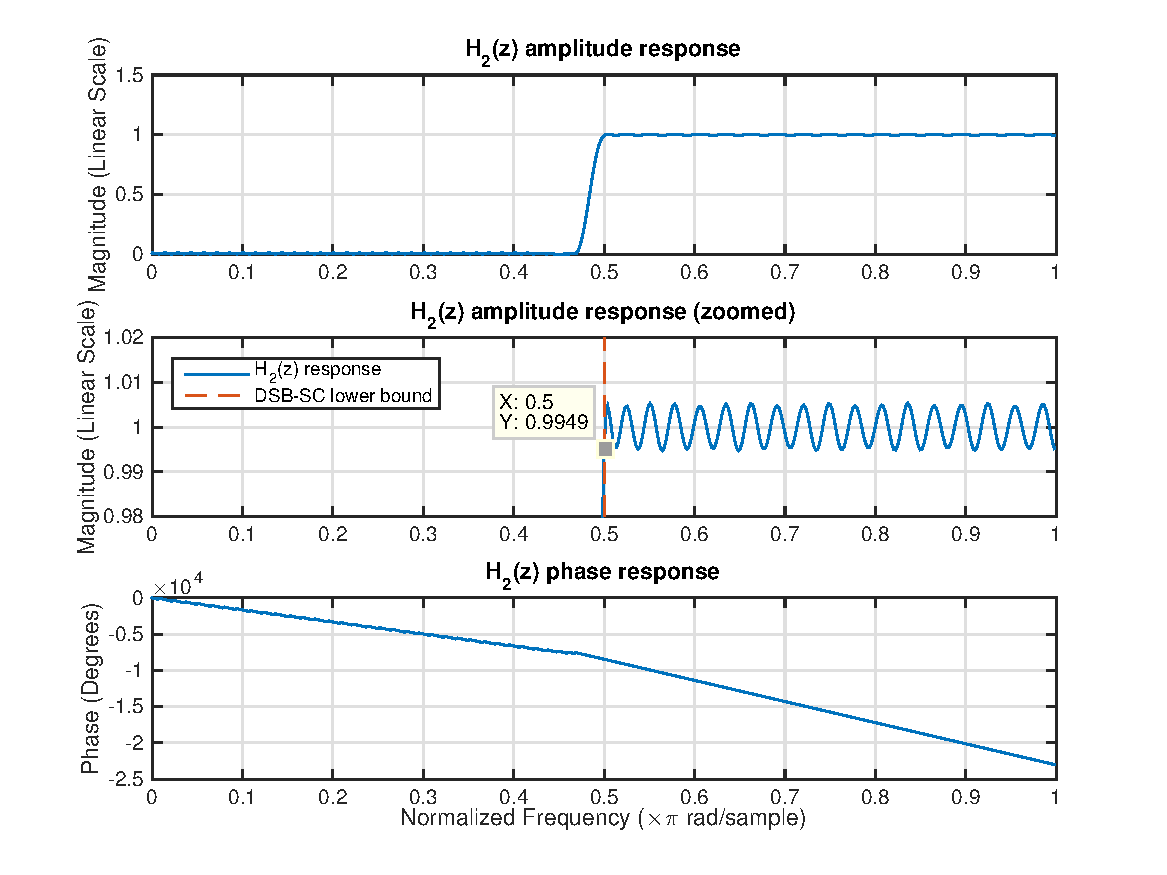
\includegraphics[width=2.5in]{H2-Response-FIR}
\caption{$H_2(z)$ Response}
\label{H2-Response-FIR}
\end{minipage}
\begin{minipage}[t]{0.33\linewidth}
\centering
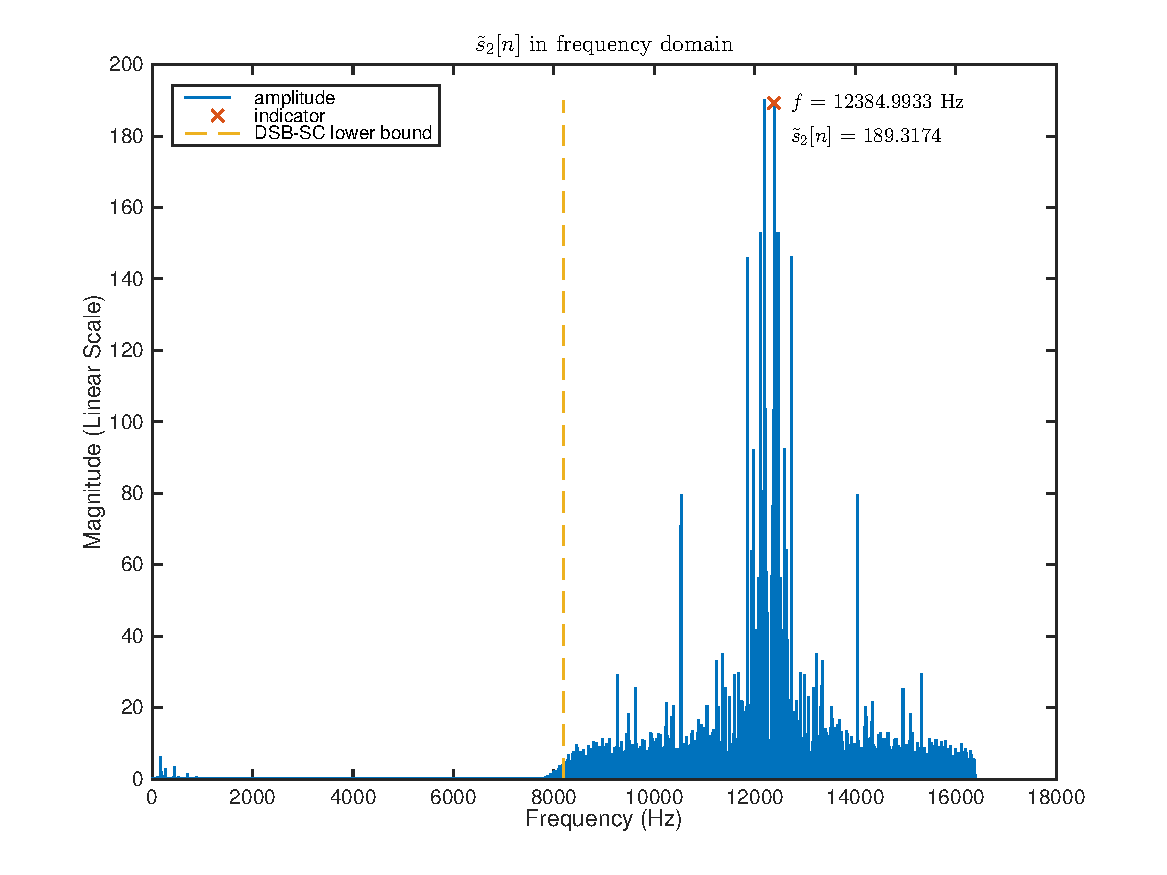
\includegraphics[width=2.5in]{s2_tilde-FIR}
\caption{$\tilde{s}_2[n]$ in frequency domain}
\label{s2_tilde-FIR}
\end{minipage}
\end{figure}

In Fig. \ref{BlockB-Response-FIR}, Block B has linear phase. In Fig. \ref{H2-Response-FIR}, $H_2(z)$ has ripple less than 0.01. In Fig. \ref{s2_tilde-FIR}, low frequency components have been successfully filtered.\\

\textbf{$H_2(z)$ is the filter obtained by cascading the filters in block A and B}.

\end{homeworkSection}

%--------------------------------------------

\begin{homeworkSection}{Block C Lowpass filter}

\subsubsection{Demodulation phase shift}
Based on the theoretical discussion on page 2, $\phi_2$ in Eq.\ref{demodulation_carrier} can be calculated by \texttt{find\_phi(s2\_tilde)} function.
\begin{equation}
\phi_2 = 0.25 \pi
\end{equation}
For instance, the spike at 12384.99 Hz in Fig. \ref{s2_tilde-FIR} corresponds to the spike at 96.99 Hz in Fig. \ref{y-FIR} (96.99 Hz + $F_c$ = 12384.99 Hz). Their magnitudes are nearly equal $189.32 \approx 189.6$ ($\frac{189.32 - 189.6}{189.32} = -0.15\%$ negligible difference). Hence, signal has been successfully demodulated.

\subsubsection{Specification}
Method: \textbf{Parks-McClellan} optimal FIR filter design\\
Passband: [0, 4096 Hz]\\
Stopband: [4596 Hz, $+\infty$)\\
Passband ripple: 0.005 (smaller than 0.01 because of cascade)\\
Stopband ripple: 0.01 (-40 dB)\\

The lowest order can be calculated by \texttt{firpmord()} function.
\begin{equation}
N = 153
\end{equation}

%--------------------------------------------

\subsubsection{Frequency Response \& Output}
\begin{figure}[H]
\begin{minipage}[t]{0.33\linewidth}
\centering
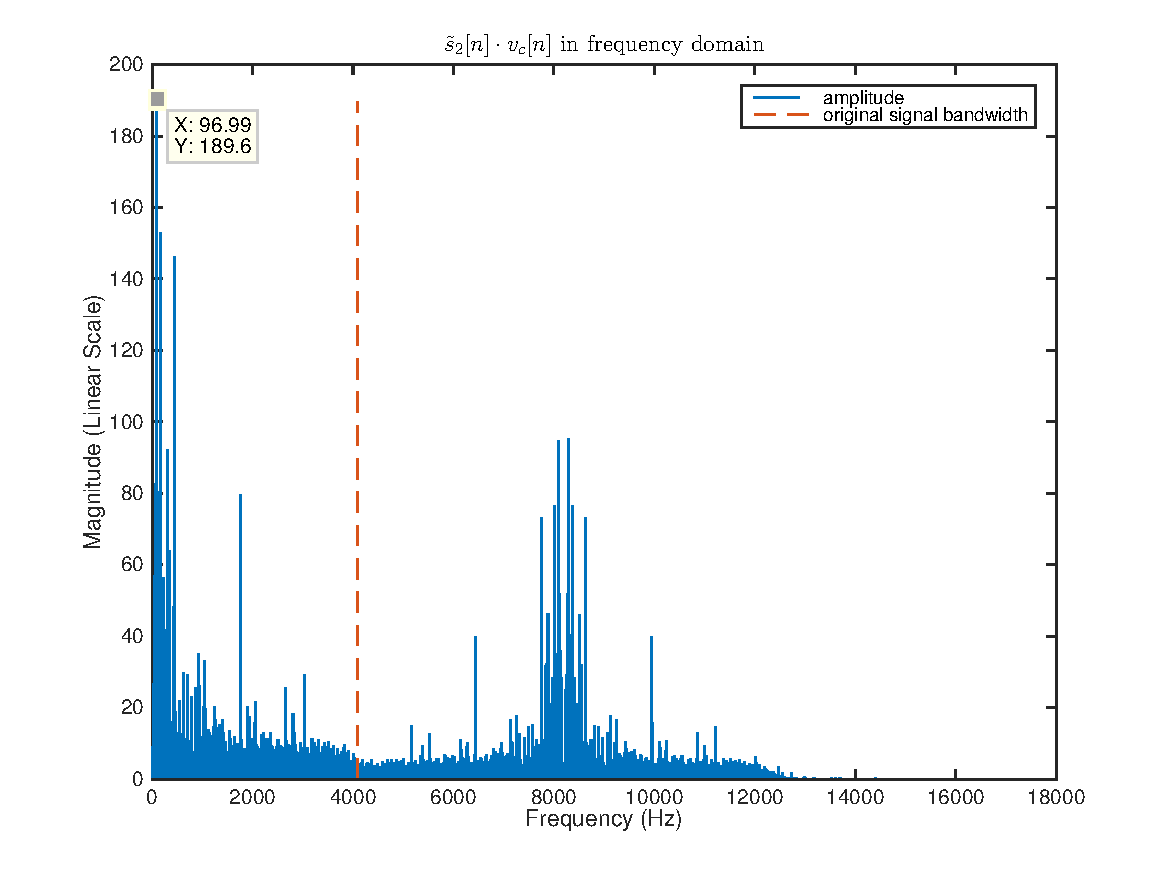
\includegraphics[width=2.5in]{y-FIR}
\caption{$\tilde{s}_2[n]$ multiplied by carrier}
\label{y-FIR}
\end{minipage}
\begin{minipage}[t]{0.33\linewidth}
\centering
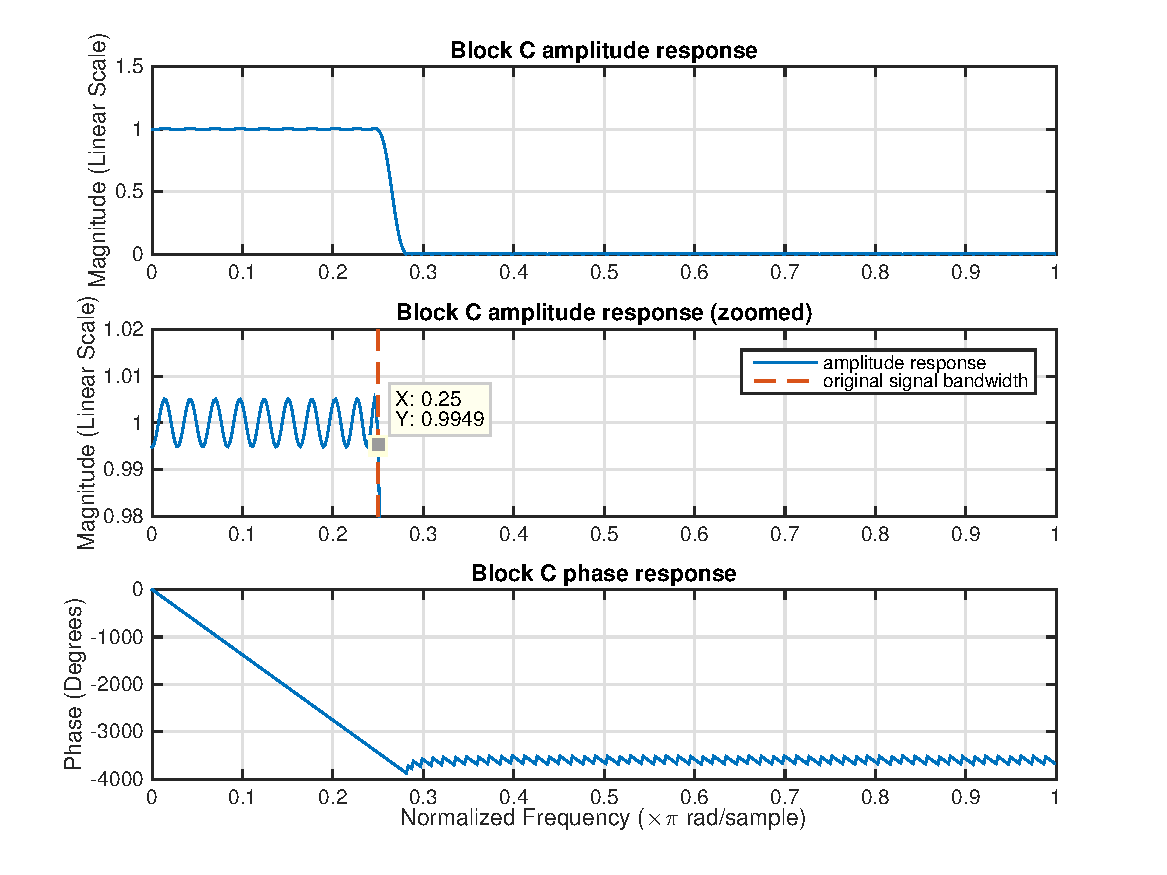
\includegraphics[width=2.5in]{BlockC-Response-FIR}
\caption{Block C response}
\label{BlockC-Response-FIR}
\end{minipage}
\begin{minipage}[t]{0.33\linewidth}
\centering
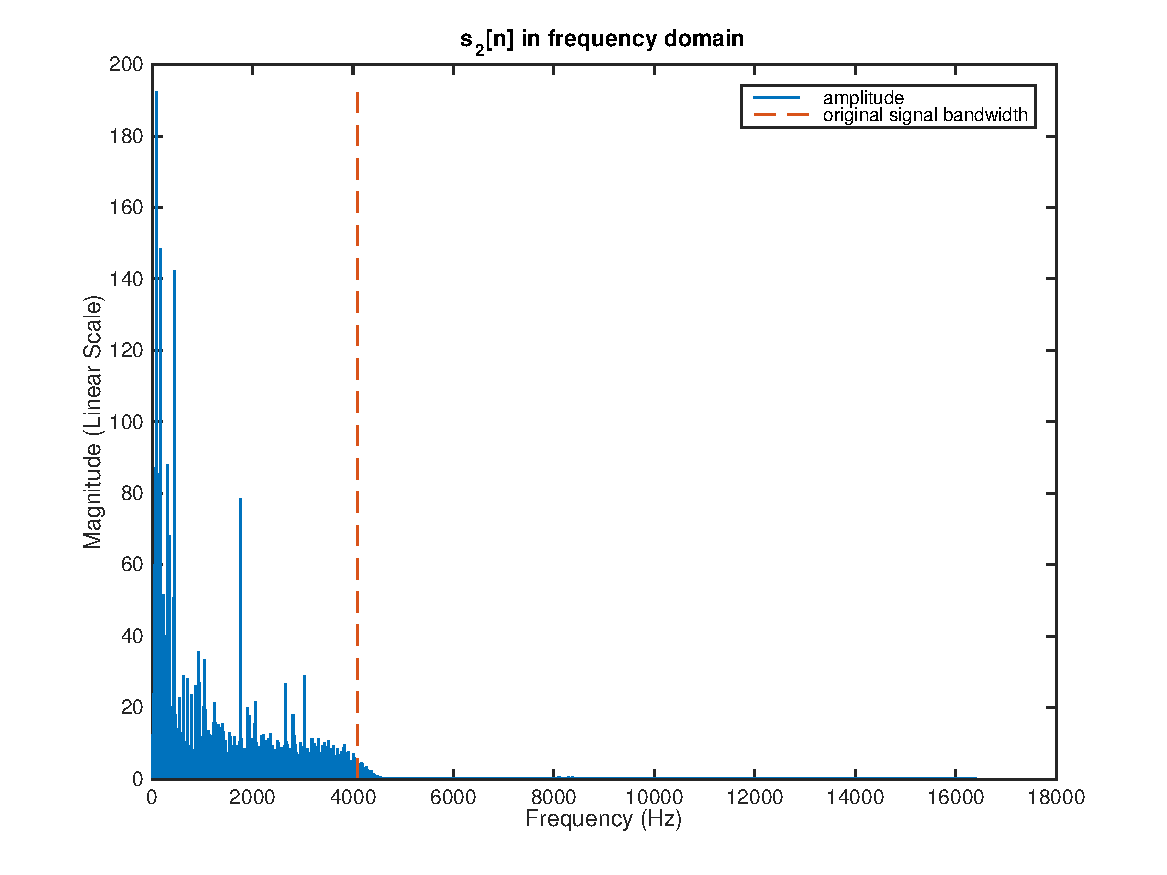
\includegraphics[width=2.5in]{s2-FIR}
\caption{$s_2[n]$ in frequency domain}
\label{s2-FIR}
\end{minipage}
\end{figure}

In Fig. \ref{BlockC-Response-FIR}, Block C has linear phase. In Fig. \ref{BlockC-Response-FIR}, block C has ripple less than 0.01. In Fig. \ref{s2-FIR}, high frequency components have been successfully filtered.

\end{homeworkSection}

%--------------------------------------------

\end{homeworkProblem}

%----------------------------------------------------------------------------------------
%	FIR filters optimization
%----------------------------------------------------------------------------------------

\begin{homeworkProblem}{FIR filters optimization}

A filter has linear phase if its frequency response can be written as
\begin{equation}
H(e^{j \omega}) = e^{-j\frac{N}{2}\omega} e^{j\beta} \breve{H}(\omega)
\end{equation}
where $N$ is the filter order and $\breve{H}(\omega)$ is a real function of $\omega$.
\begin{equation}
\theta(\omega) = \beta - \frac{N}{2}\omega
\end{equation}
Group delay
\begin{equation}
\tau_g(\omega) = - \frac{d\theta(\omega)}{d\omega} = \frac{N}{2}
\end{equation}

\begin{homeworkSection}{Total group delays}
\begin{align*}
H_1(z):\ &N = 184 + 141 = 325 \longrightarrow \tau_g = \frac{325}{2} = 162.5\\
\text{ABC cascade}:\ &N = 184 + 140 + 153 = 477 \longrightarrow \tau_g = \frac{477}{2} = 238.5
\end{align*}
\end{homeworkSection}

%--------------------------------------------

\begin{homeworkSection}{Total group delays minimization}
Minimizing total filter orders is to minimize total group delays because of the proportional relationship.\\

Filter order can be reduced from two aspects.\\
1. expand transition region\\
2. make full use of the ripple range
\end{homeworkSection}

%--------------------------------------------

\begin{homeworkSection}{New Specifications}
\subsubsection{Block A}
Passband: [0, 6472.8 Hz] and [8272.8 Hz, $+\infty$)\\
Stopband: [7371.8 Hz, 7373.8 Hz]\\
Passband ripple: 0.005\\
Stopband ripple: 0.001 (-60 dB)

\subsubsection{Block B}
Stopband: [0, 4096 Hz]\\
Passband: [8192 Hz, $+\infty$)\\
Stopband ripple: 0.01 (-40 dB)\\
Passband ripple: 0.005

\subsubsection{Block C \& D}
Passband: [0, 4096 Hz]\\
Stopband: [8192 Hz, $+\infty$)\\
Passband ripple: 0.01 (-40 dB)\\
Stopband ripple: 0.005
\end{homeworkSection}

\begin{homeworkSection}{Minimal total group delays}
\begin{align*}
H_1(z):\ &N = 102 + 16 = 118 \longrightarrow \tau_g = \frac{118}{2} = 59\\
\text{ABC cascade}:\ &N = 102 + 16 + 18 = 136 \longrightarrow \tau_g = \frac{136}{2} = 68
\end{align*}\end{homeworkSection}

\begin{homeworkSection}{Frequency response}
\begin{figure}[H]
\begin{minipage}[t]{0.5\linewidth}
\centering
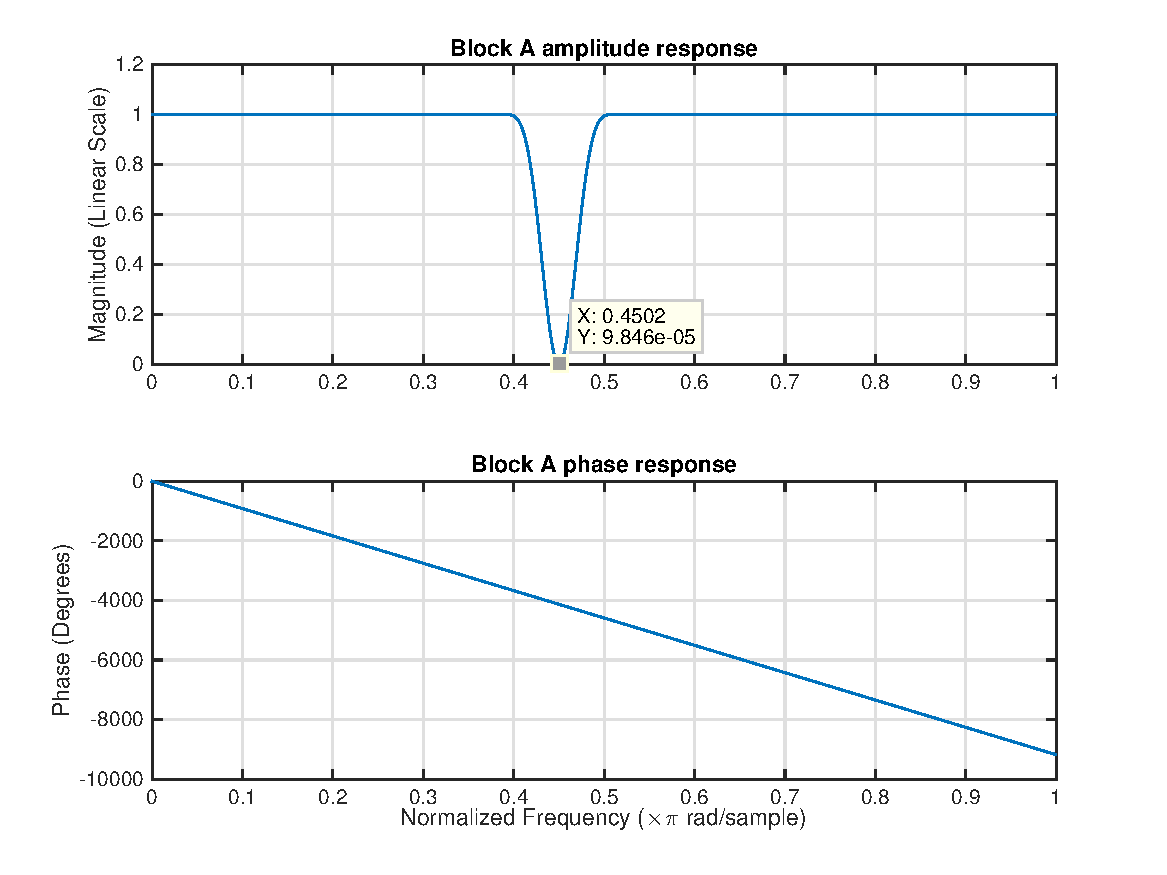
\includegraphics[width=3.3in]{BlockA-Response-FIR-min}
\caption{Block A response}
\label{BlockA-Response-FIR-min}
\end{minipage}
\begin{minipage}[t]{0.5\linewidth}
\centering
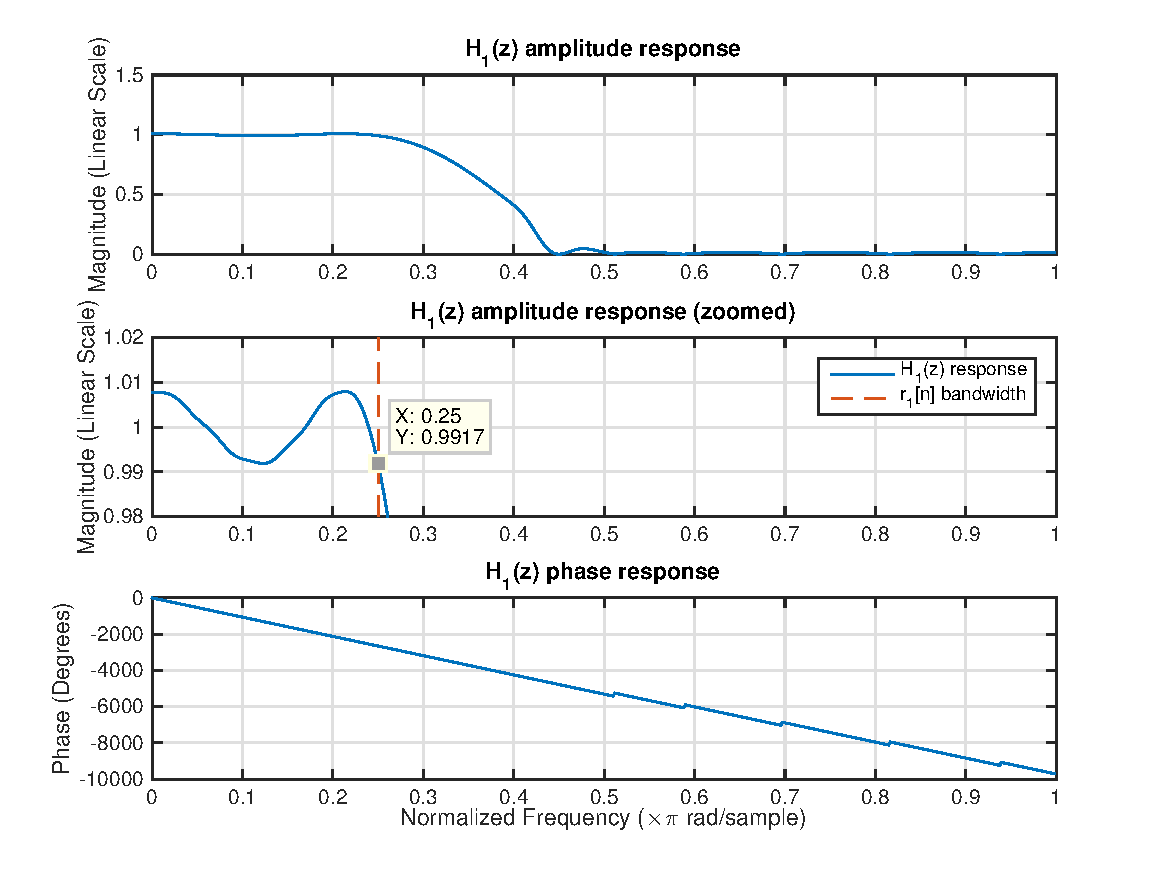
\includegraphics[width=3.3in]{H1-Response-FIR-min}
\caption{$H_1(z)$ Response}
\label{H1-Response-FIR-min}
\end{minipage}
\end{figure}

\begin{figure}[H]
\begin{minipage}[t]{0.5\linewidth}
\centering
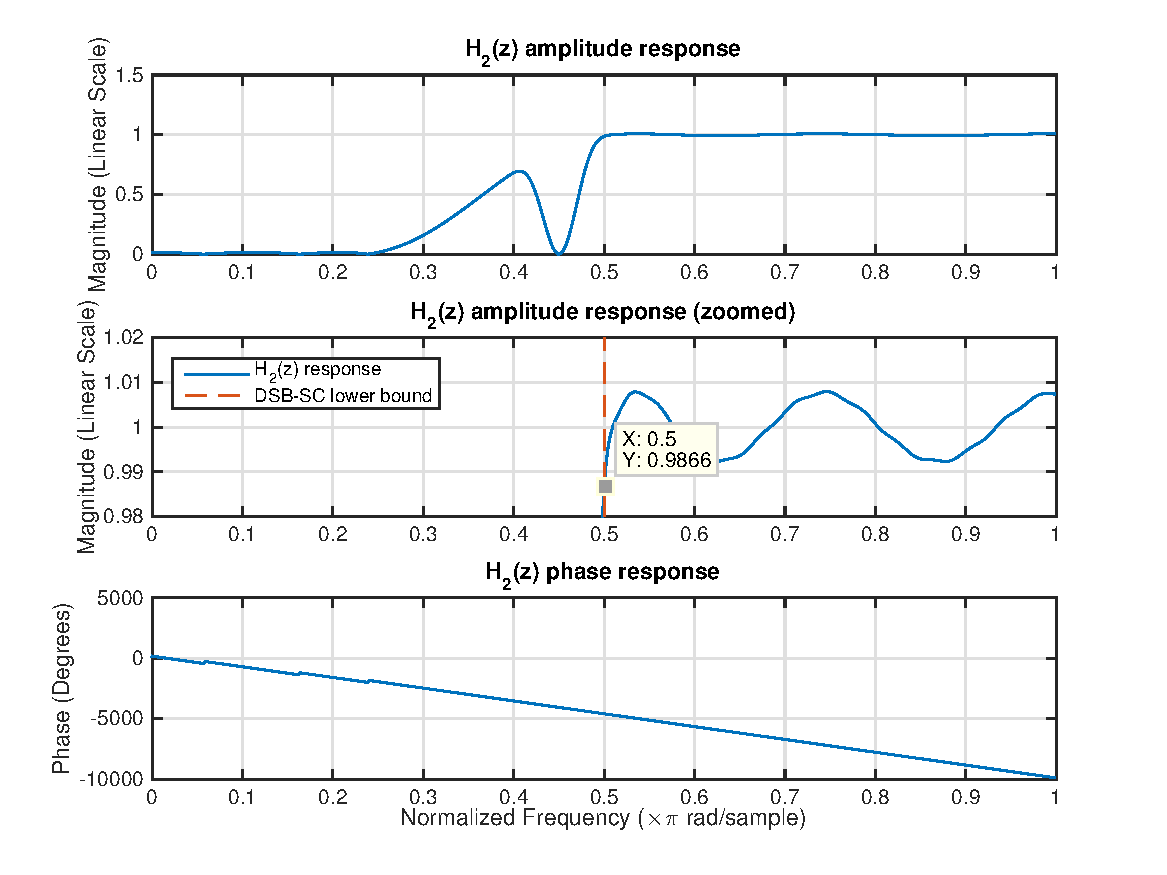
\includegraphics[width=3.3in]{H2-Response-FIR-min}
\caption{$H_2(z)$ Response}
\label{H2-Response-FIR-min}
\end{minipage}
\begin{minipage}[t]{0.5\linewidth}
\centering
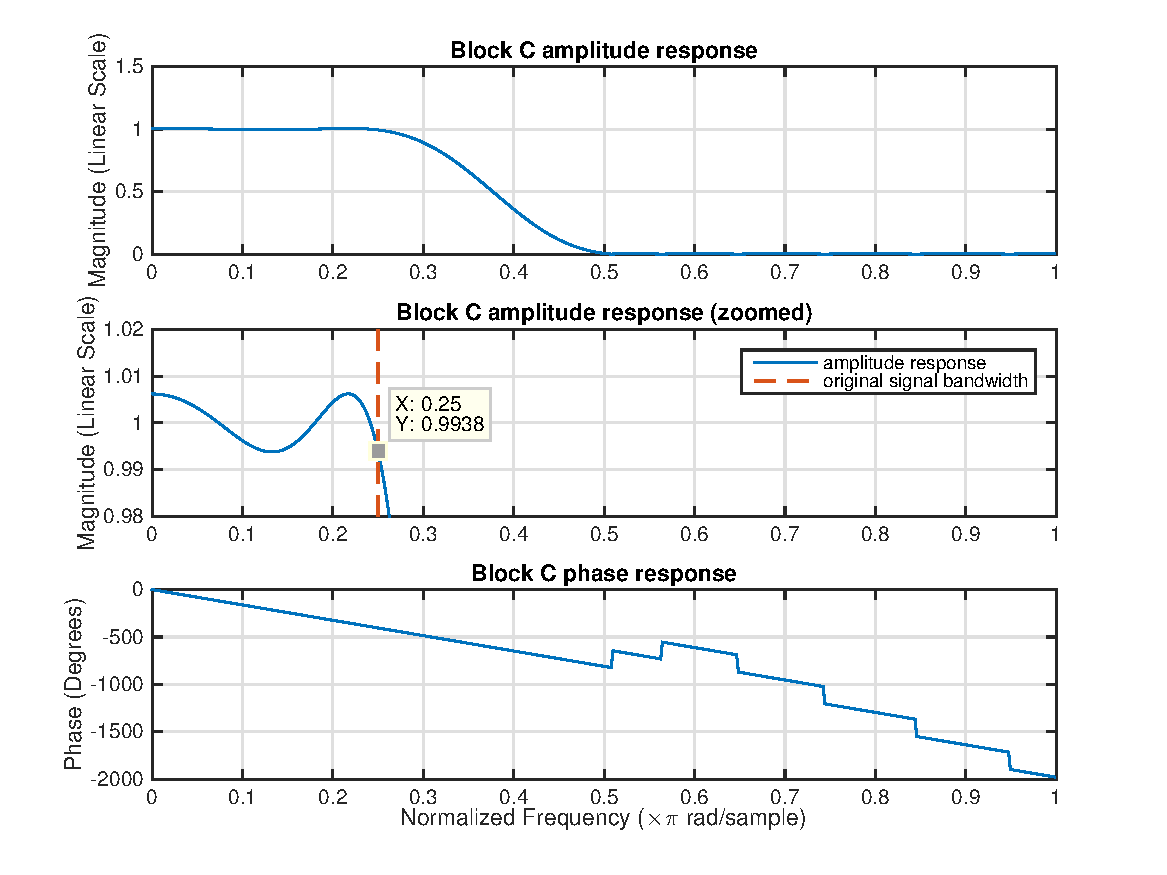
\includegraphics[width=3.3in]{BlockC-Response-FIR-min}
\caption{Block C response}
\label{BlockC-Response-FIR-min}
\end{minipage}
\end{figure}

In Fig. \ref{BlockA-Response-FIR-min}, attenuation $20 \log_{10}(9.846 \times 10^{-5})$ = -80.1348 dB $<$ -60 dB. In Fig. \ref{H1-Response-FIR-min}, the maximal ripple of $H_1(z)$ is $1 - 0.9917 = 0.0083 < 0.01$. In Fig. \ref{H2-Response-FIR-min} and Fig. \ref{BlockC-Response-FIR-min}, even in the worst situation, the maximal ripple of ABC cascade is $1 - 0.9866 \times 0.9938 = 0.0195 < 2\%$.
\end{homeworkSection}

%--------------------------------------------

\end{homeworkProblem}

%----------------------------------------------------------------------------------------
%	IIR filters design
%----------------------------------------------------------------------------------------

\begin{homeworkProblem}{IIR filters design}

%--------------------------------------------

\begin{homeworkSection}{Block A 2nd order notch filter}

\begin{equation}
H_{BS}(z) = \frac{1+\alpha}{2} \frac{1-2\beta z^{-1} + z^{-2}}{1 - \beta (1+\alpha) z^{-1} + \alpha z^{-2}}
\end{equation}

We have known the notch frequency $\omega_0 = 0.45\pi \text{ rad/sample}$,
\begin{equation}
\beta = \cos(\omega_0) = \textbf{0.156434}
\end{equation}

We set
\begin{equation}
B_w = \cos^{-1}(\frac{2\alpha}{1+\alpha^2}) = 0.005 \pi \text{ rad/sample}
\end{equation}
Given $0<\alpha<1$
\begin{equation}
\alpha = \frac{1}{\cos(B_w)} - \sqrt{\frac{1}{(\cos(B_w))^2}-1} = \textbf{0.984414}
\end{equation}

\begin{figure}[H]
\begin{minipage}[t]{0.5\linewidth}
\centering
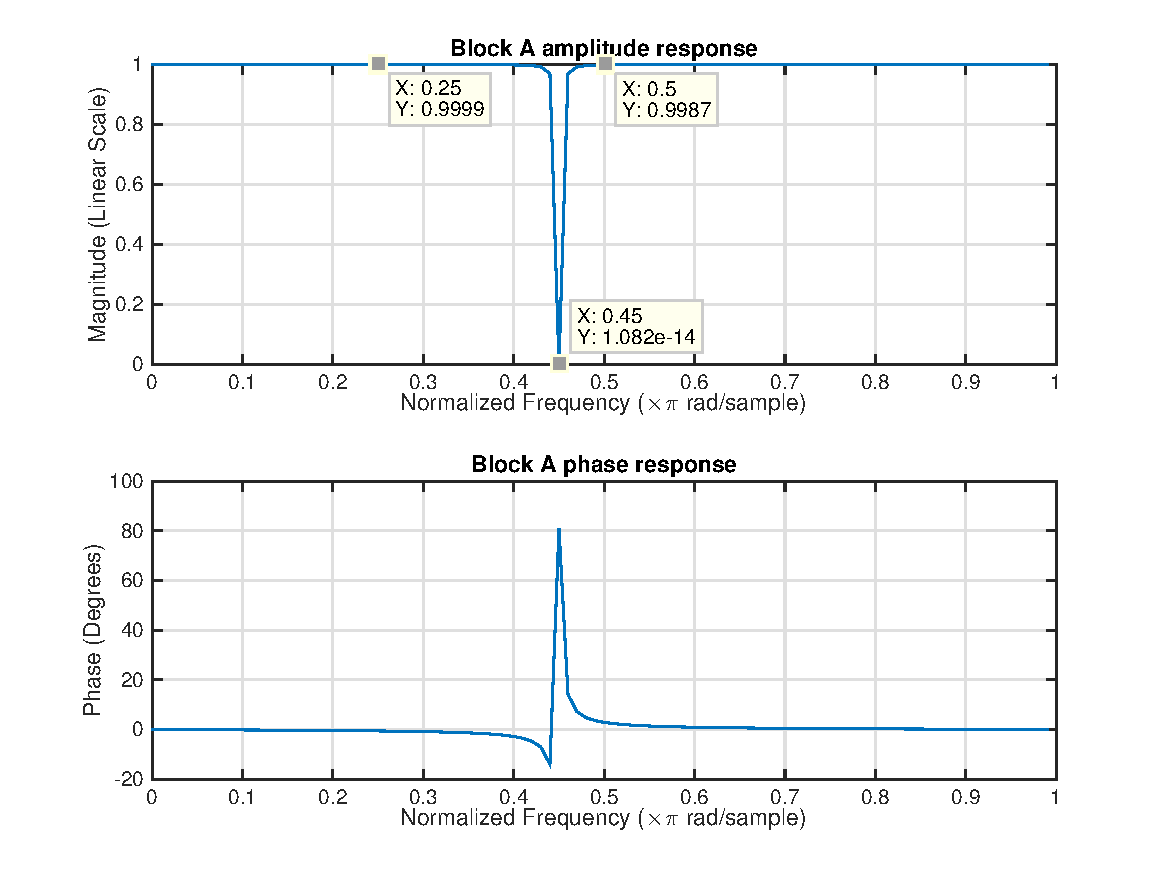
\includegraphics[width=3.3in]{BlockA-Response}
\caption{Block A response}
\label{BlockA-Response}
\end{minipage}
\begin{minipage}[t]{0.5\linewidth}
\centering
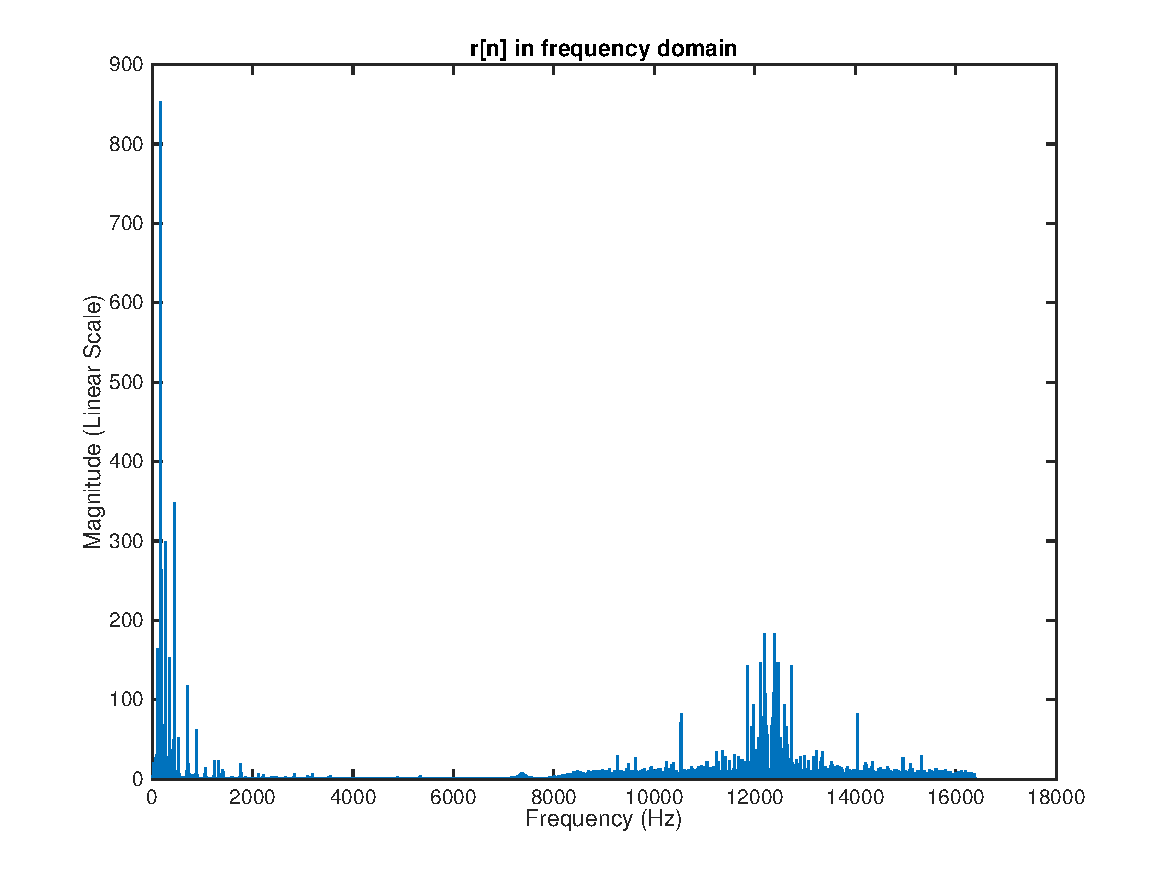
\includegraphics[width=3.3in]{r_FFT}
\caption{$r[n]$ in frequency domain}
\label{r_FFT}
\end{minipage}
\end{figure}

As can be seen in Figure \ref{BlockA-Response} and Figure \ref{r_FFT}, $w[n]$ at 7372.8 Hz ($0.45\pi$ rad/sample) has been attenuated by $20 \log_{10}(1.082 \times 10^{-14})$ = -279.3155 dB, hence the design satisfies the -60 dB gain requirement. In addition, the notch filter has gain of 0.9999 and 0.9987 at $0.25\pi$ rad/sample and $0.5\pi$ rad/sample respectively.
\begin{equation}\label{A025}
A_{0.25\pi} = 0.9999
\end{equation}
\begin{equation}\label{A05}
A_{0.5\pi} = 0.9987
\end{equation}
Due to the monotonicity, in the bands of [0, 4096 Hz] and [8192 Hz, $+\infty$), these two ripples are maxima.

\end{homeworkSection}

%--------------------------------------------

\begin{homeworkSection}{Block D Lowpass filter}

%--------------------------------------------

\subsubsection{Specification}
Model: \textbf{Chebyshev Type I}\\
Passband ripple: 0.0099 (explained by Eq. \ref{ripple-blockD})\\
Stopband attenuation: 0.001 (-60 dB)\\
Passband: [0, $0.25\pi$ rad/sample]\\
Stopband: [$0.255\pi$ rad/sample, $\pi$ rad/sample)\\

The total ripple for the frequency band occupied by $r_1[n]$ must be less than 0.01. The gain of block A at $0.25\pi$ rad/sample is 0.9999 (Eq. \ref{A025}). Hence, the ripple of block D is
\begin{equation}\label{ripple-blockD}
1 - \frac{1 - 0.01}{0.9999} = 0.0099
\end{equation}

The lowest order can be calculated by \texttt{cheb1ord()} function.
\begin{equation}
N = 15
\end{equation}

%--------------------------------------------

\subsubsection{Frequency Response \& Output}
\begin{figure}[H]
\begin{minipage}[t]{0.33\linewidth}
\centering
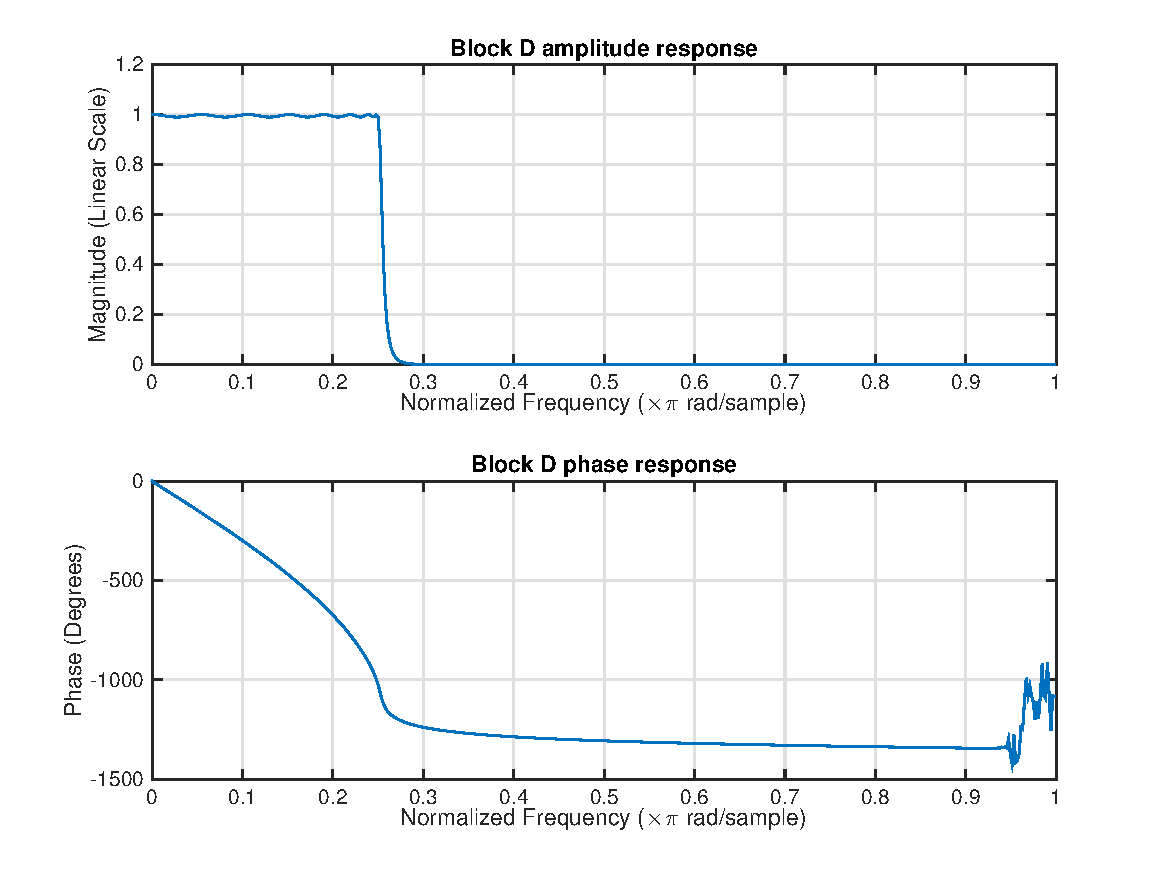
\includegraphics[width=2.5in]{BlockD-Response}
\caption{Block D response}
\label{BlockD-Response}
\end{minipage}
\begin{minipage}[t]{0.33\linewidth}
\centering
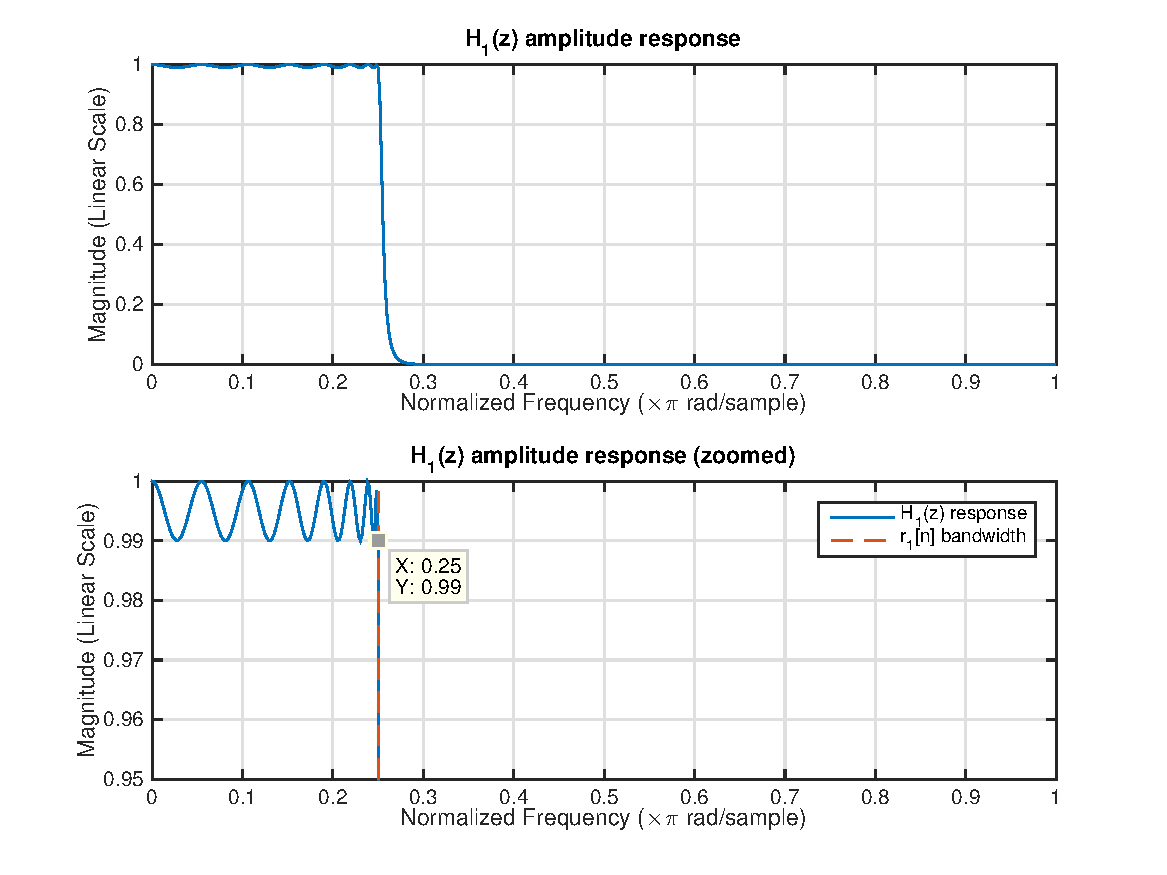
\includegraphics[width=2.5in]{H1-Response}
\caption{$H_1(z)$ Response}
\label{H1-Response}
\end{minipage}
\begin{minipage}[t]{0.33\linewidth}
\centering
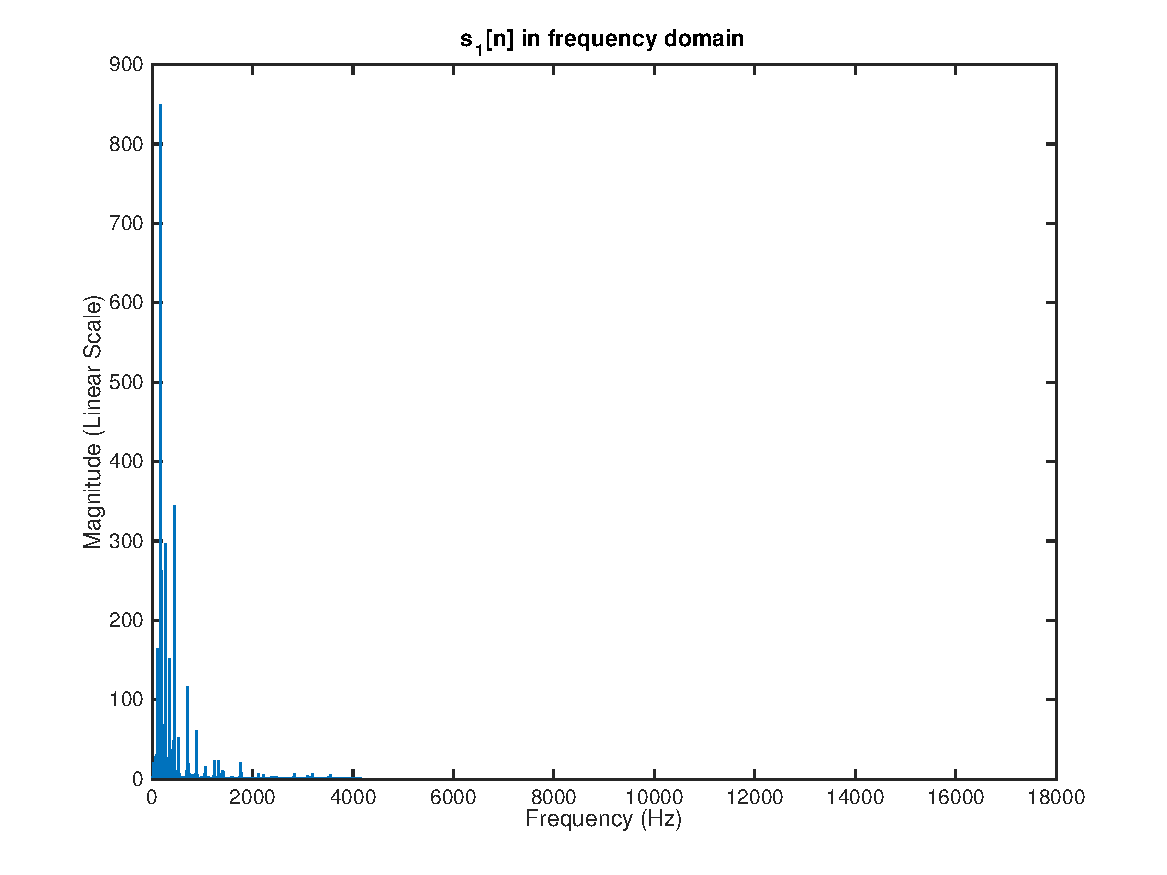
\includegraphics[width=2.5in]{s1}
\caption{$s_1[n]$ in frequency domain}
\label{s1}
\end{minipage}
\end{figure}

In Fig. \ref{H1-Response}, $H_1(z)$ has ripple less than 0.01. In Fig. \ref{s1}, high frequency components have been successfully filtered.

\end{homeworkSection}

%--------------------------------------------

\begin{homeworkSection}{Block B Highpass filter}

\subsubsection{Specification}
Model: \textbf{Butterworth}\\
Stopband attenuation: 0.001 (-60 dB)\\
Passband ripple: 0.0088 (explained by Eq. \ref{ripple-cascade} and Eq. \ref{ripple-blockA})\\
Stopband: [0, $0.45\pi$ rad/sample]\\
Passband: [$0.5\pi$ rad/sample, $\pi$ rad/sample)\\

\textbf{$H_2(z)$ is the filter obtained by cascading the filters in block A and B}.\\

We specify the ripple of $H_2(z)$ and the ripple of block C are both 0.01.

\begin{equation}\label{ripple-cascade}
1 - (1-0.01) \times (1-0.01) = 0.0199 < 2\%
\end{equation}

As a result, the total ripple for the cascade of the filters in block A, B and C is such that the the magnitude spectrum of the demodulated signal $s_2[n]$ is within 2\% of the magnitude of the original signal (the one which was modulated) for each frequency.\\

Given the gain of block A at $0.5\pi$ rad/sample is 0.9987 (Eq. \ref{A05}), the ripple of block B is
\begin{equation}\label{ripple-blockA}
1 - \frac{1 - 0.01}{0.9987} = 0.0088
\end{equation}

The lowest order can be calculated by \texttt{buttord()} function.
\begin{equation}
N = 57
\end{equation}

%--------------------------------------------

\subsubsection{Frequency Response \& Output}
\begin{figure}[H]
\begin{minipage}[t]{0.33\linewidth}
\centering
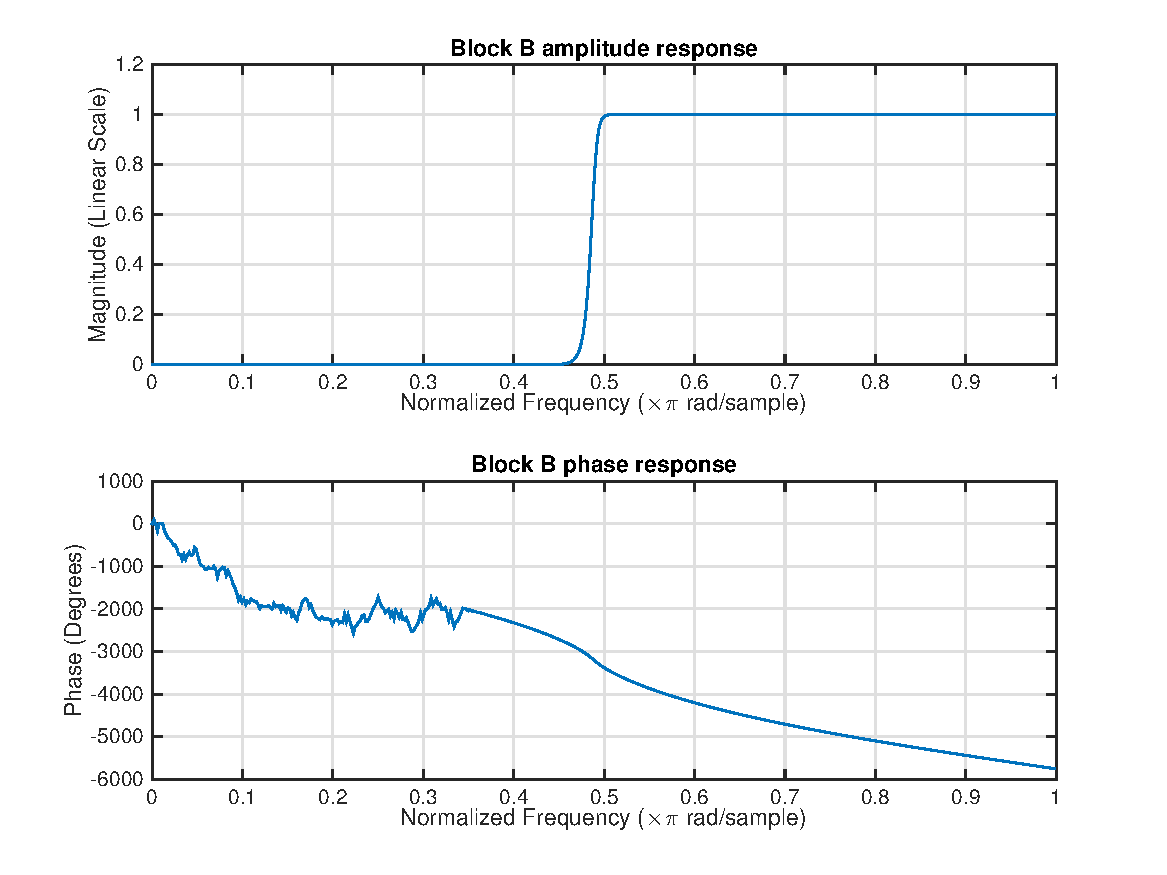
\includegraphics[width=2.5in]{BlockB-Response}
\caption{Block B response}
\label{BlockB-Response}
\end{minipage}
\begin{minipage}[t]{0.33\linewidth}
\centering
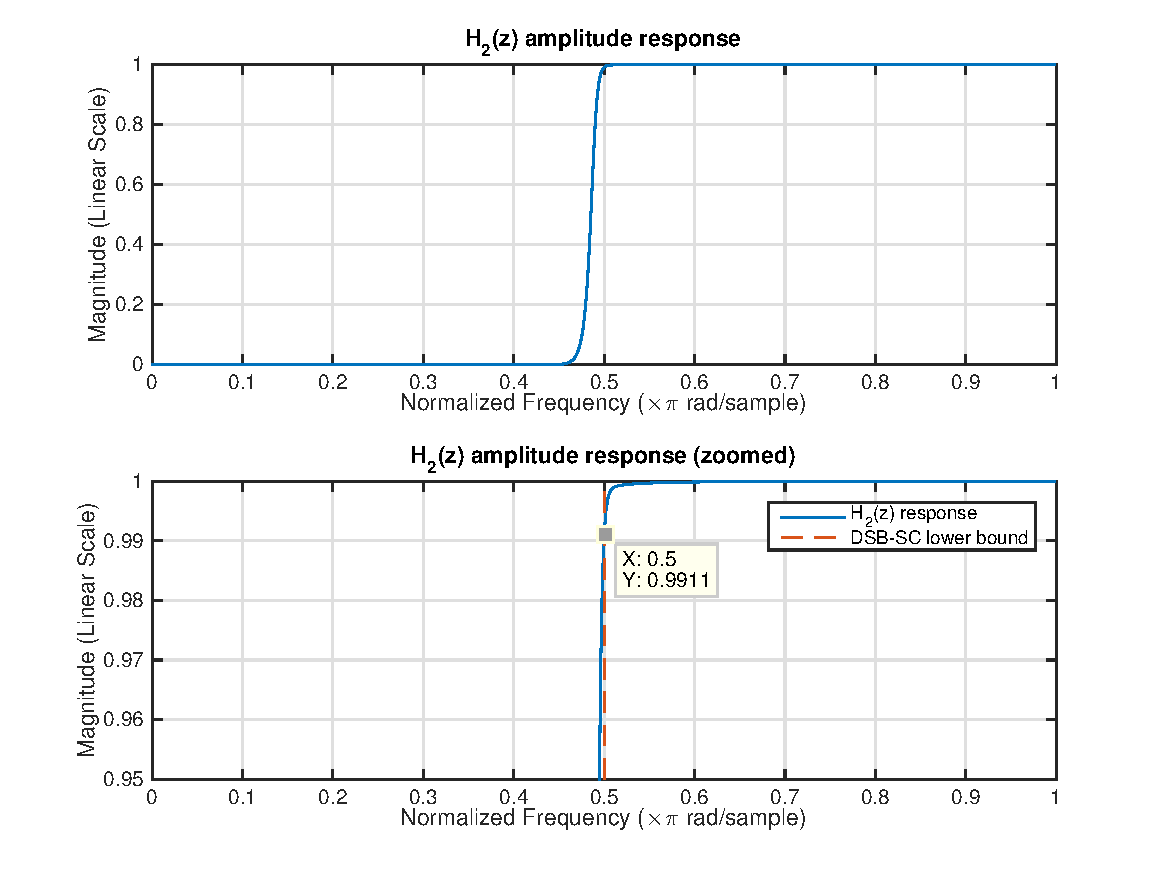
\includegraphics[width=2.5in]{H2-Response}
\caption{$H_2(z)$ Response}
\label{H2-Response}
\end{minipage}
\begin{minipage}[t]{0.33\linewidth}
\centering
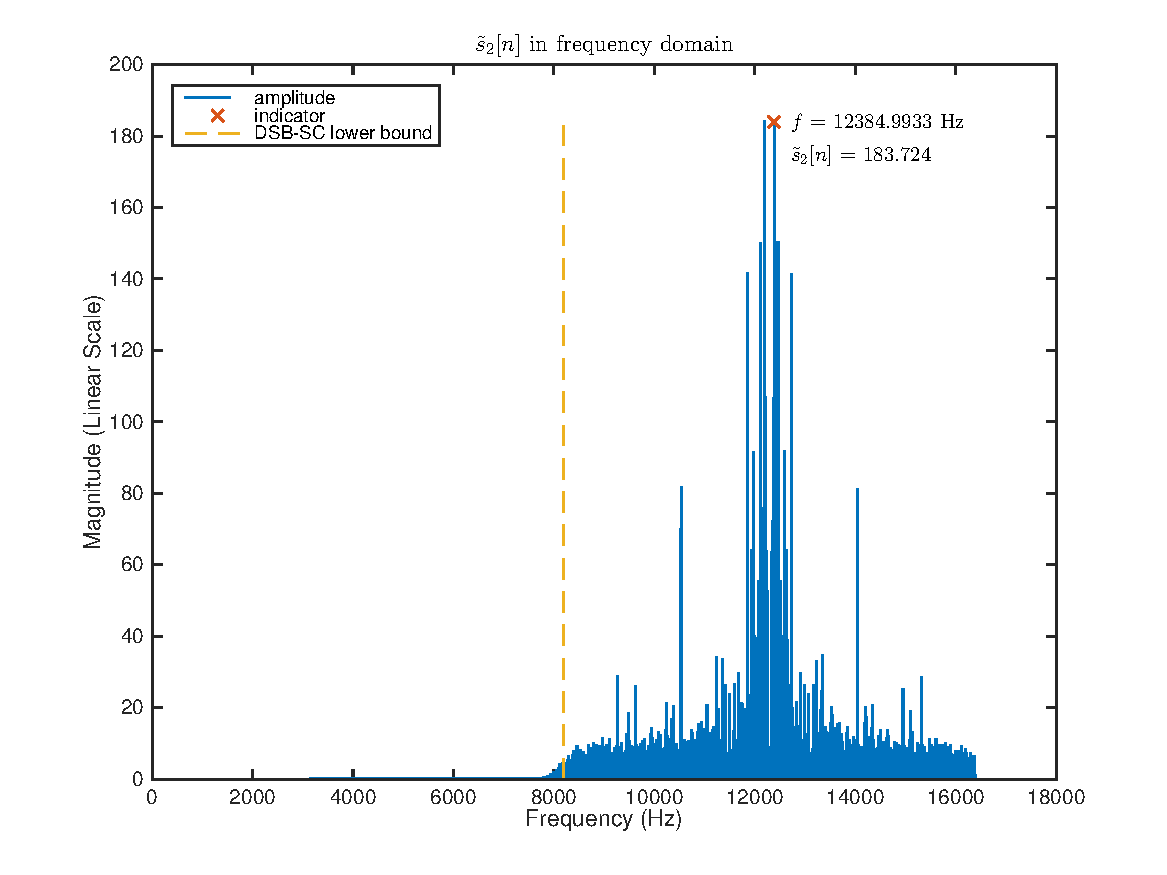
\includegraphics[width=2.5in]{s2_tilde}
\caption{$\tilde{s}_2[n]$ in frequency domain}
\label{s2_tilde}
\end{minipage}
\end{figure}

In Fig. \ref{H2-Response}, $H_2(z)$ has ripple less than 0.01. In Fig. \ref{s2_tilde}, low frequency components have been successfully filtered.

\end{homeworkSection}

%--------------------------------------------

\begin{homeworkSection}{Block C Lowpass filter}

\subsubsection{Demodulation phase shift}
Based on the theoretical discussion on page 2, $\phi_2$ in Eq.\ref{demodulation_carrier} can be calculated by \texttt{find\_phi(s2\_tilde)} function.
\begin{equation}
\phi_2 = 0.45 \pi
\end{equation}
For instance, the spike at 12384.99 Hz in Fig. \ref{s2_tilde} corresponds to the spike at 96.99 Hz in Fig. \ref{y} (96.99 Hz + $F_c$ = 12384.99 Hz). Their magnitudes are nearly equal $183.724 \approx 183.8$ ($\frac{183.724 - 183.8}{183.724} = -0.041\%$ negligible difference). Hence, signal has been successfully demodulated.

\subsubsection{Specification}
Model: \textbf{Elliptic}\\
Passband ripple: 0.01 (Eq. \ref{ripple-cascade})\\
Stopband attenuation: 0.001 (-60 dB)\\
Passband: [0, $0.25\pi$ rad/sample]\\
Stopband: [$0.255\pi$ rad/sample, $\pi$ rad/sample)\\

The lowest order can be calculated by \texttt{ellipord()} function.
\begin{equation}
N = 11
\end{equation}

%--------------------------------------------

\subsubsection{Frequency Response \& Output}
\begin{figure}[H]
\begin{minipage}[t]{0.33\linewidth}
\centering
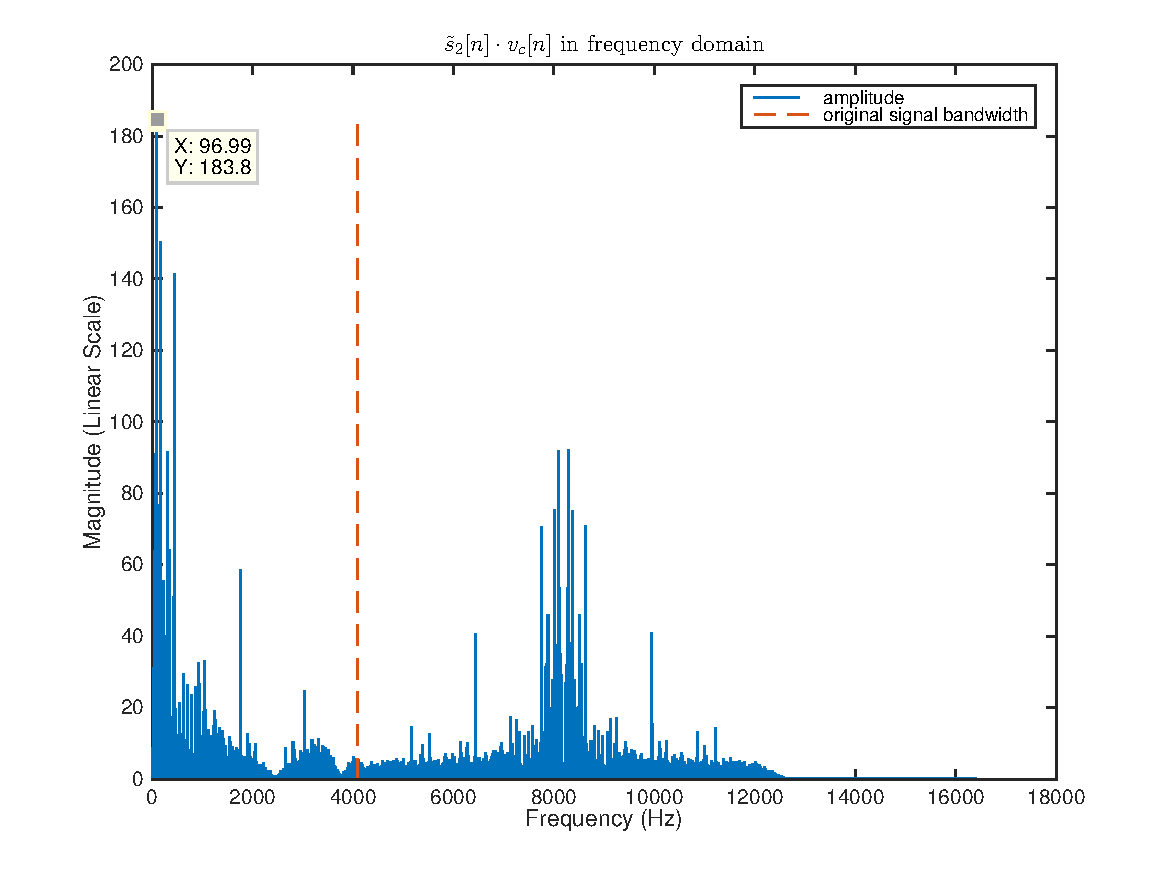
\includegraphics[width=2.5in]{y}
\caption{$\tilde{s}_2[n]$ multiplied by carrier}
\label{y}
\end{minipage}
\begin{minipage}[t]{0.33\linewidth}
\centering
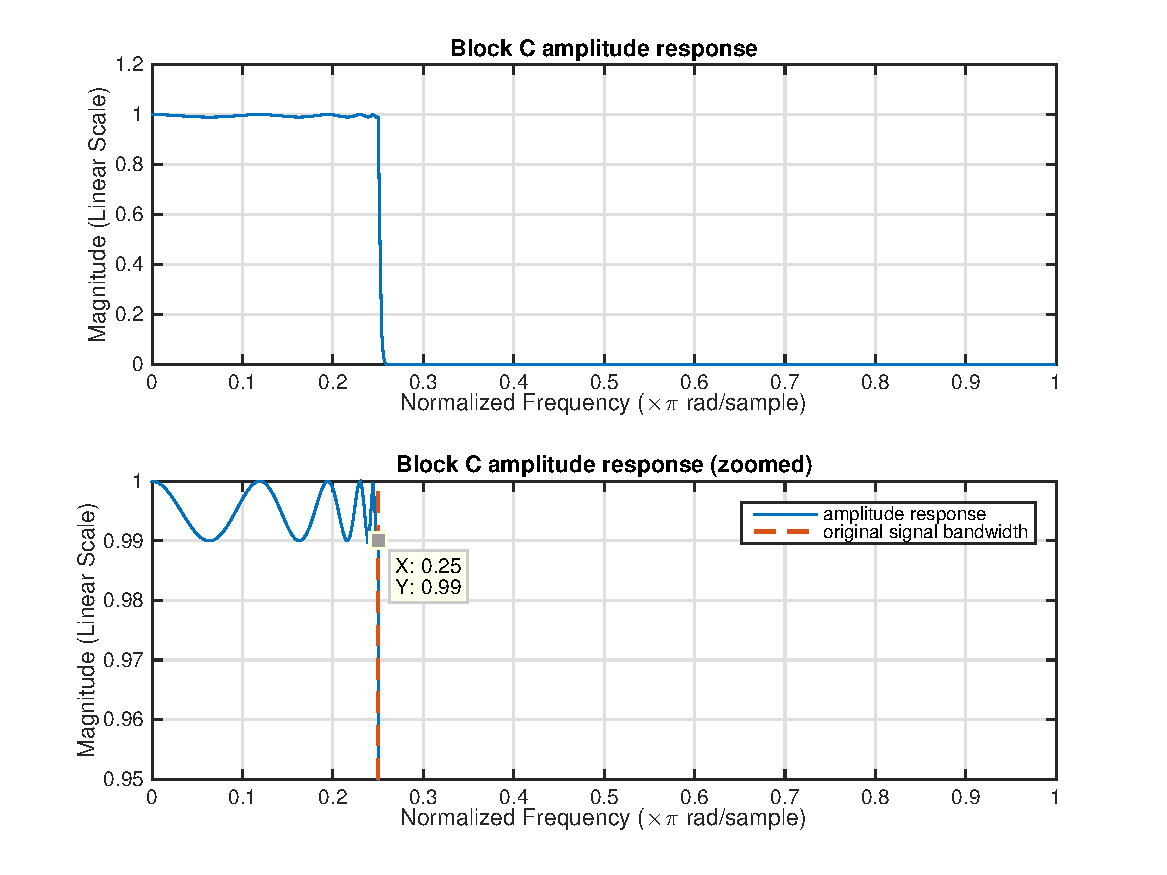
\includegraphics[width=2.5in]{BlockC-Response}
\caption{Block C response}
\label{BlockC-Response}
\end{minipage}
\begin{minipage}[t]{0.33\linewidth}
\centering
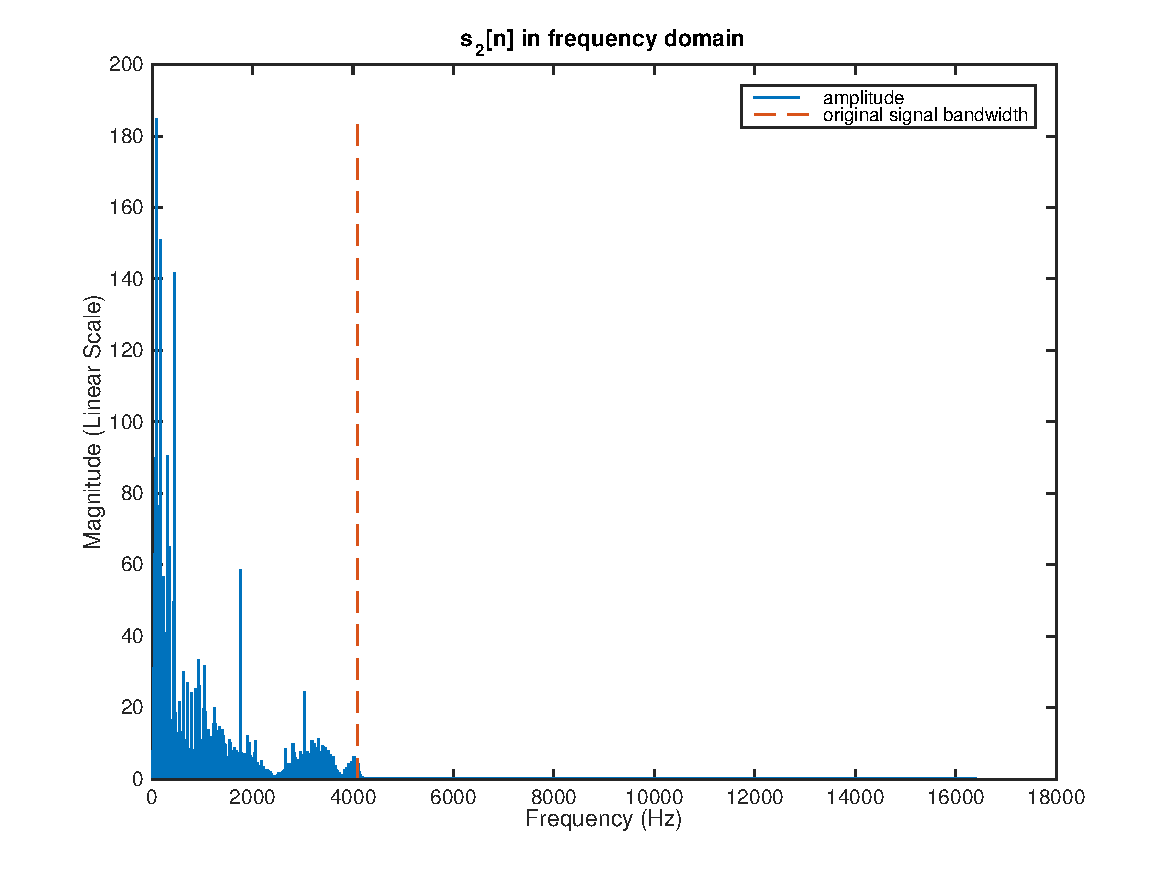
\includegraphics[width=2.5in]{s2}
\caption{$s_2[n]$ in frequency domain}
\label{s2}
\end{minipage}
\end{figure}

In Fig. \ref{BlockC-Response}, block C has ripple less than 0.01. In Fig. \ref{s2}, high frequency components have been successfully filtered.

\end{homeworkSection}

%--------------------------------------------

\end{homeworkProblem}

%----------------------------------------------------------------------------------------
%	FIR and IIR comparison
%----------------------------------------------------------------------------------------

\begin{homeworkProblem}{FIR and IIR comparison}

%--------------------------------------------

\begin{homeworkSection}{Filter parameters comparison}

\begin{table}[!hbp]
\centering
\begin{tabu} to 0.8\textwidth {X[l] X[c] X[c]}
                            &FIR  & IIR \\
Passband edge frequency     & Yes & Yes \\
Stopband edge frequency     & Yes & Yes \\
Passband desired amplitudes & Yes &     \\
Stopband desired amplitudes & Yes &     \\
Stopband attenuation        &     & Yes \\
Passband ripple             & Yes & Yes \\
Stopband ripple             & Yes &    
\end{tabu}
\caption{Parameters Comparison}
\end{table}

FIR can control the desired amplitude more accurately and flexibly at the cost of more parameters required. Besides, FIR requires one more parameter to control stopband ripple.

\end{homeworkSection}

%--------------------------------------------

\begin{homeworkSection}{Sound quality comparison}
In order to compare, we recorded some speech and compared the outputs of FIR and IIR in a continuous loop. We realized output from IIR filters was more close to the original sound. However, IIR filtering was more time-consuming due to larger filter orders. We thought IIR filters have inherent advantages in terms of sound quality because of \textbf{linear phase}.\\

When input is $e^{j2\pi f_0 t}$, output is
\begin{equation}
|H(f_0)| e^{j2\pi f_0 t + \angle H(f_0)} = |H(f_0)| e^{j2\pi f_0 (t + \frac{\angle H(f_0)}{2\pi f_0})}
\end{equation}
i.e. output is proportion to input delayed by $-\frac{\angle H(f_0)}{2\pi f_0}$ seconds = \textit{phase delay}.\\

If phase response is not linear, this depends on $f_0$.\\
i.e. system delays Fourier components of inputs by different amounts, depending on frequency. Signal will be distorted.
\end{homeworkSection}

%--------------------------------------------

\end{homeworkProblem}

%----------------------------------------------------------------------------------------
%	IIR filters optimization
%----------------------------------------------------------------------------------------

\begin{homeworkProblem}{IIR filters optimization}

%--------------------------------------------

\begin{homeworkSection}{Methods to minimize filter orders}
Filter order can be reduced from three aspects.\\
1. change filter type\\
2. expand transition region\\
3. make full use of the ripple range
\end{homeworkSection}

%--------------------------------------------

\begin{homeworkSection}{New Specifications}
\subsubsection{Block B}
Model: \textbf{Elliptic}\\
Stopband: [0, $0.25\pi$ rad/sample]\\
Passband: [$0.5\pi$ rad/sample, $\pi$ rad/sample)\\
Stopband attenuation: 0.001 (-60 dB)\\
Passband ripple: 0.0088

\subsubsection{Block C \& D}
Model: \textbf{Elliptic}\\
Passband: [0, $0.25\pi$ rad/sample]\\
Stopband: [$0.5\pi$ rad/sample, $\pi$ rad/sample)\\
Passband ripple: 0.0100 (C), 0.0099 (D)\\
Stopband attenuation: 0.001 (-60 dB)
\end{homeworkSection}

%--------------------------------------------

\begin{homeworkSection}{Minimal total filter orders}
\begin{align*}
H_1(z):\ &N = 2 + 5 = 7\\
\text{ABC cascade}:\ &N = 2 + 5 + 5 = 12
\end{align*}
\end{homeworkSection}

%--------------------------------------------

\begin{homeworkSection}{Frequency response}
\begin{figure}[H]
\begin{minipage}[t]{0.33\linewidth}
\centering
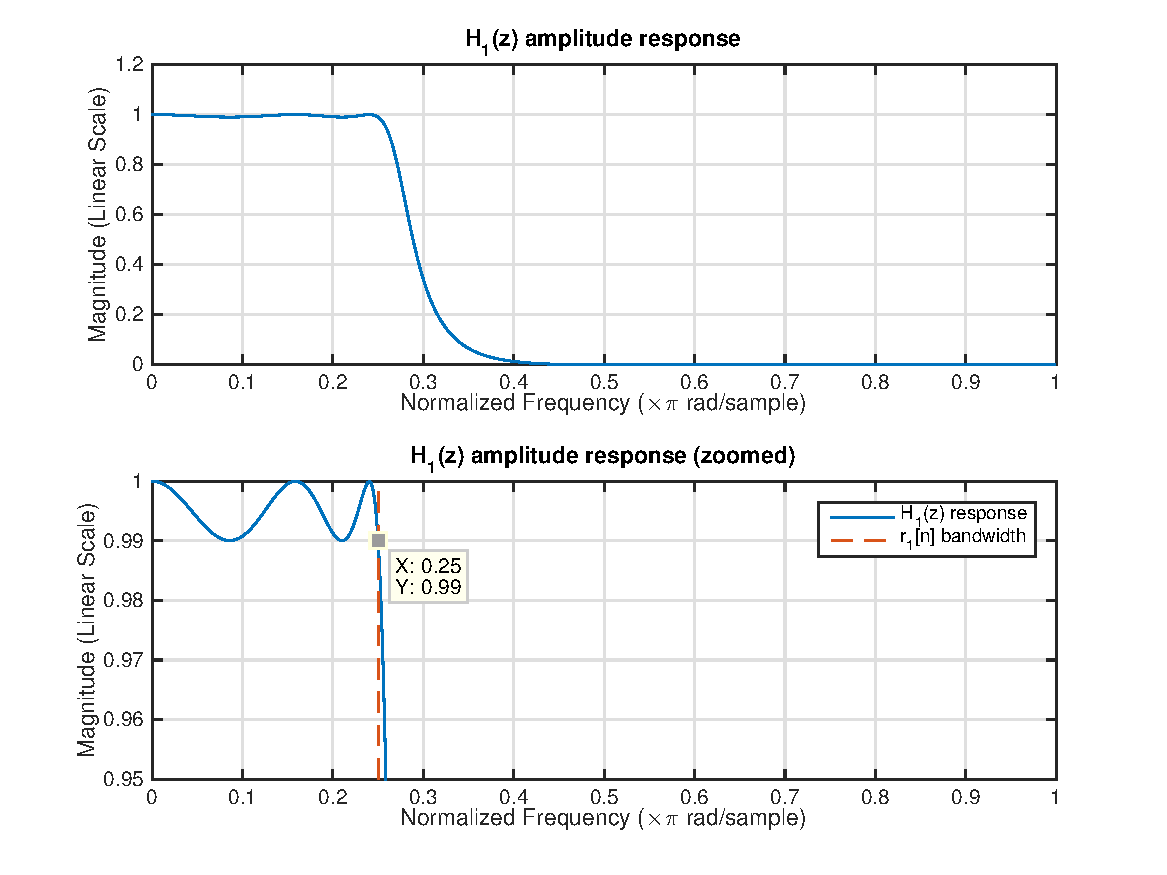
\includegraphics[width=2.5in]{H1-Response-min}
\caption{$H_1(z)$ Response}
\label{H1-Response-min}
\end{minipage}
\begin{minipage}[t]{0.33\linewidth}
\centering
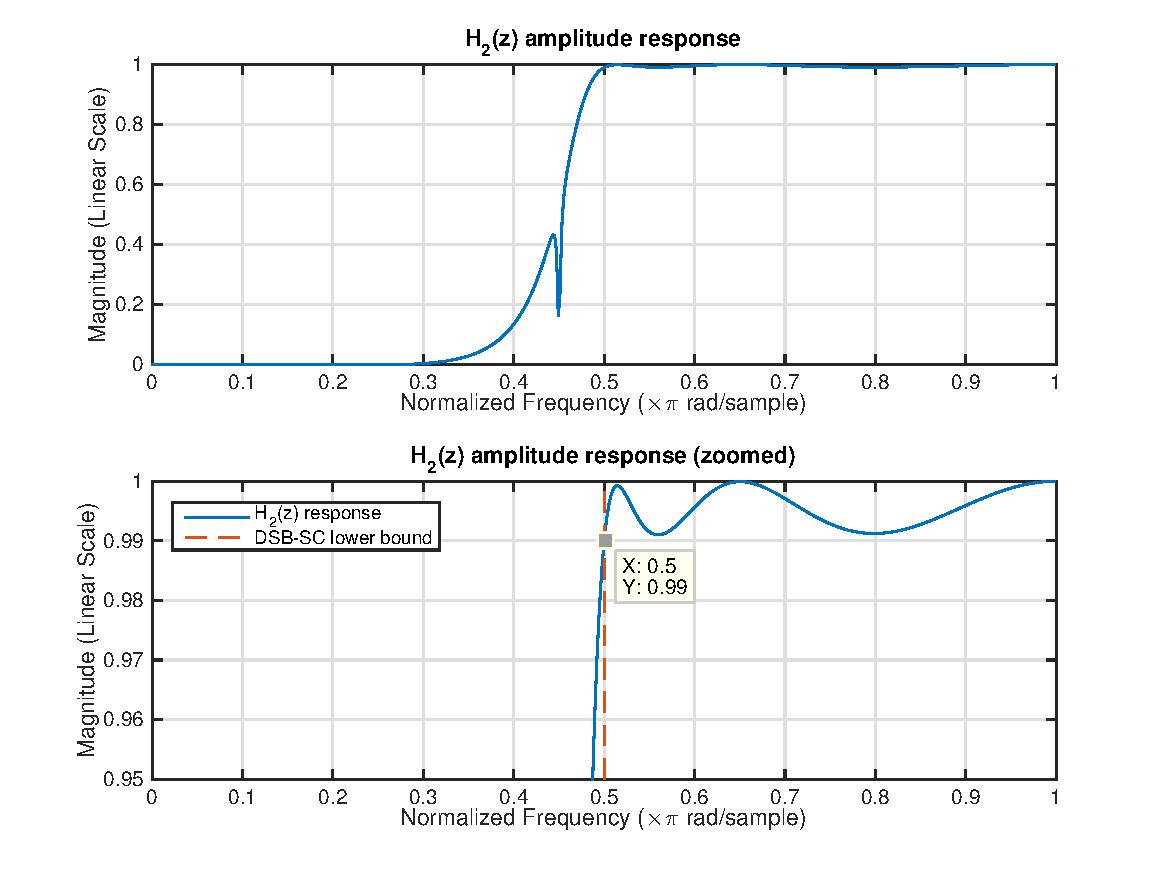
\includegraphics[width=2.5in]{H2-Response-min}
\caption{$H_2(z)$ Response}
\label{H2-Response-min}
\end{minipage}
\begin{minipage}[t]{0.33\linewidth}
\centering
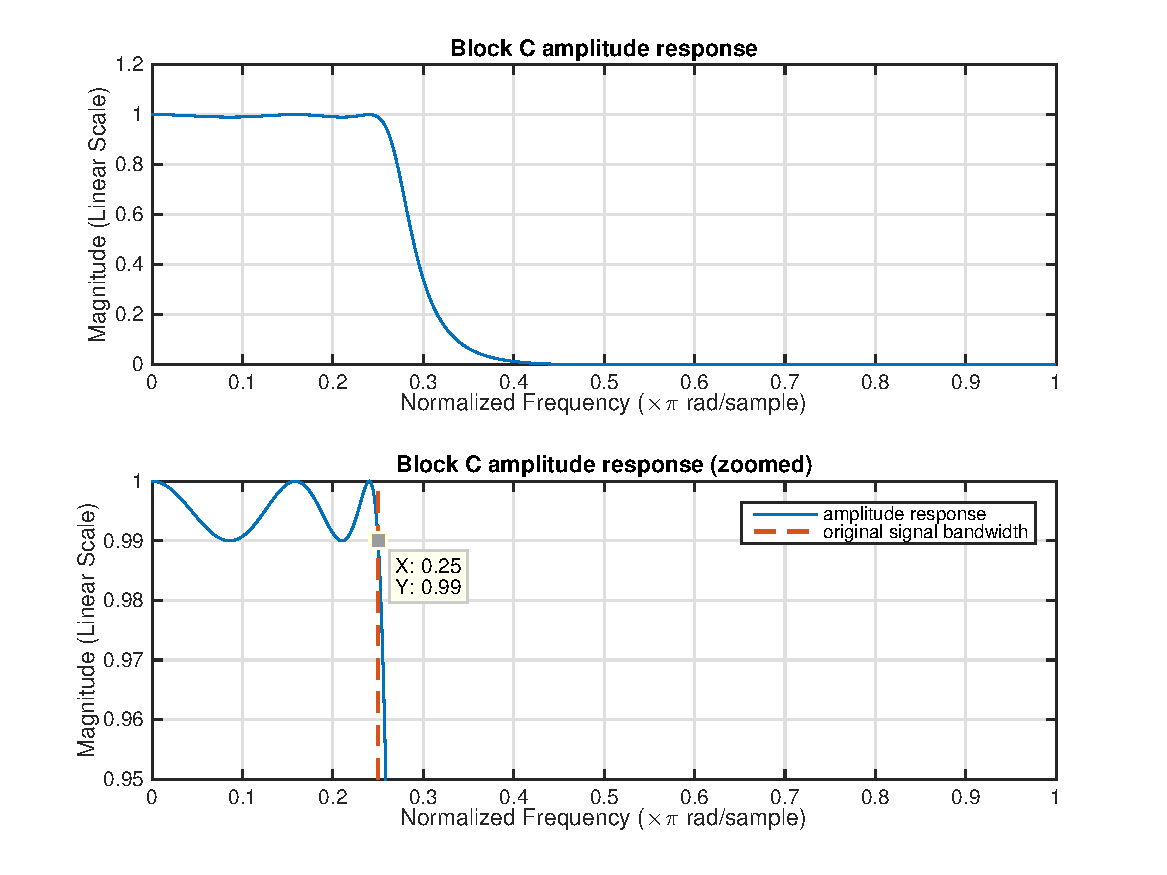
\includegraphics[width=2.5in]{BlockC-Response-min}
\caption{Block C response}
\label{BlockC-Response-min}
\end{minipage}
\end{figure}

In Fig. \ref{H1-Response-min}, the maximal ripple of $H_1(z)$ is $1 - 0.99 = 0.01$. In Fig. \ref{H2-Response-min} and Fig. \ref{BlockC-Response-min}, even in the worst situation, the maximal ripple of ABC cascade is $1 - 0.99 \times 0.99 = 0.0199 < 2\%$.
\end{homeworkSection}

%--------------------------------------------

\end{homeworkProblem}

%----------------------------------------------------------------------------------------
%	Appendix
%----------------------------------------------------------------------------------------

\newpage
\section*{Appendix}

\subsection*{\texttt{find\_phi(s2\_tilde)}}\label{find_phi}
\lstinputlisting{find_phi.m}

\subsection*{\texttt{single\_side\_FFT(x, F\_s)}}
\lstinputlisting{single_side_FFT.m}

\subsection*{\texttt{analysis.m}}
\lstinputlisting{analysis.m}

\subsection*{\texttt{FIR.m}}
\lstinputlisting{FIR.m}

\subsection*{\texttt{IIR.m}}
\lstinputlisting{IIR.m}

% \subsection*{\texttt{FIR\_minimized.m}}
% \lstinputlisting{FIR_minimized.m}

% \subsection*{\texttt{IIR\_minimized.m}}
% \lstinputlisting{IIR_minimized.m}

%----------------------------------------------------------------------------------------

\end{document}
